 %
% File acl2018.tex
%
%% Based on the style files for ACL-2017, with some changes, which were, in turn,
%% Based on the style files for ACL-2015, with some improvements
%%  taken from the NAACL-2016 style
%% Based on the style files for ACL-2014, which were, in turn,
%% based on ACL-2013, ACL-2012, ACL-2011, ACL-2010, ACL-IJCNLP-2009,
%% EACL-2009, IJCNLP-2008...
%% Based on the style files for EACL 2006 by 
%%e.agirre@ehu.es or Sergi.Balari@uab.es
%% and that of ACL 08 by Joakim Nivre and Noah Smith

\documentclass[11pt,a4paper]{article}
\usepackage[hyperref]{acl2018}
\usepackage{times}
\usepackage{latexsym}
\usepackage{booktabs}
\usepackage{url}
\usepackage{amsmath}	% for \begin{align}
\usepackage{graphicx}	% for \includegraphics{filename}
\usepackage{subcaption}	% for \begin{subfigure}[t]{0.5\textwidth}
\usepackage{courier}	% for \texttt{}

\usepackage{amsmath,amssymb} % prevent misalignment tab character?

\aclfinalcopy % Uncomment this line for the final submission
%\def\aclpaperid{***} %  Enter the acl Paper ID here

%\setlength\titlebox{5cm}
% You can expand the titlebox if you need extra space
% to show all the authors. Please do not make the titlebox
% smaller than 5cm (the original size); we will check this
% in the camera-ready version and ask you to change it back.

\newcommand\BibTeX{B{\sc ib}\TeX}

\title{Adaptive Beam Search in Sequence-to-Sequence Models}

\author{Yu-Hsiang Lin \quad Shuxin Lin \quad Hai Pham \\
  Language Technologies Institute \\
  Carnegie Mellon University \\
%   Affiliation / Address line 3 \\
{\tt\small $\left\{yuhsianl, shuxinl, htpham\right\}$@andrew.cmu.edu}
%   {\tt email@domain} 
%   \\\And
%   Second Author \\
%   Affiliation / Address line 1 \\
%   Affiliation / Address line 2 \\
%   Affiliation / Address line 3 \\
%   {\tt email@domain} \\
  }

\date{}

\begin{document}
\maketitle
\begin{abstract}
% We plan to apply new techniques such as combining dynamical beam size with trainable beam search to boost up the training and test-time decoding of the sequence-to-sequence model. We review the related approaches, and report our work in replicating state-of-the-art results.
Natural language processing tasks usually require to decode the most likely output sequence which involves searching through all the possible output sequences based on their likelihood. Beam search is a heuristic search algorithm used in the test-time decoding of sequence-to-sequence model. While it might have an advantage over greedy search for accuracy, it leads to time and resource hunger due to keeping and searching through a fixed amount of beams at each step as the beam size increases. We aim to address this problem and propose methods of adapting the beam size for decoding with help of deterministic agent and reinforcement learning, in particular for the \textit{decoding phase} in Seq2Seq model. In the experiments we show that the proposed adaptive beam search strategies yield better results on two NLP tasks compared with baseline models.
\end{abstract}

%%%%%%%%%%%%%%%%%%%%%%%%%%%%%%%%%
%         INTRODUCTION              
%%%%%%%%%%%%%%%%%%%%%%%%%%%%%%%%%
\section{Introduction} \label{sec:introduction}
Since its invention, sequence-to-sequence model (Seq2Seq) \cite{seq2seq_2014} has been a go-to model for many translation-related tasks,  % probably more examples needed 
especially since the advent of attention model \cite{bahdanau2014neural,luong2015effective}. Despite its great successes in many domains, how to train and decode seq2seq model is still an open problem because of the drawback of traditional maximum likelihood training which is, most of the cases, unable to find the maximum-a-posteriori of a to-be-decoded single sentence over the whole corpus. 

Amongst many heuristic approaches to remediate that problem, \textit{greedy search} and \textit{beam search} are the most popular. While greedy search is known for its lightweight, elegant characteristics, beam search is generally better in practice by considering not only the best-scored word at each time step but maintaining a window of best words. 
% In this project, we will be addressing the disadvantages of previous approaches for seq2seq using beam search and proposing an improvement for it in training and decoding phases. We also present our results on the Name Entity Recognition task.
In this paper, we will revisit recent researches on related topic in Section 2 and address the disadvantages of previous Seq2seq model using beam search and introduce our improvement with attention in Section 3. Our novel dynamic beam search algorithms will be discussed in Section 4 and 5. We also present our experimental results and analysis in Section 6 and 7	.
%%%%%%%%%%%%%%%%%%%%%%%%%%%%%%%%%
%         RELATED WORK              
%%%%%%%%%%%%%%%%%%%%%%%%%%%%%%%%%
\section{Related Work} \label{sec:related_work}% Literature Review 
The straightforward approach to improve seq2seq model trained with the traditional maximum likelihood method  of ground truths is to improve the decoding phase. While beam search is considered the de-factor approach \cite{seq2seq_2014}, greedy search, if designed properly, can yield a comparable performance, if not better in some cases, while having a much more lightweight architecture. \citet{goyal2017differentiable} proposed an approximated version of greedy search over the scheduled sampling training procedure \cite{bengio2015scheduled}. 
%% PROBABLY NEED MORE REFERENCE for REINFORCE
% Reinforcement learning 
Unlike tackling with decoding phase solely, another useful approach to improve seq2seq is to design a better architecture or technique of helping decode right on the training phase. One widely-employed approach is to 
%is to avoid the low performance of greedy search and high delay of beam search, 
convert it into an imitation learning problem \cite{daume2009search,ross2011reduction,bengio2015scheduled} where expert guidance from human is injected to make the agent more robust and efficient. 
A naturally connected method is to use reinforcement learning \cite{sutton1998reinforcement} which employs a reward-based loss instead of maximum likelihood-based \cite{ranzato2015sequence, gu2017learning}, giving rise to a new family of techniques which is fitted to the discrete text domain. 

% Reinforcement learning
While discriminative training is the straightforward method for seq2seq training, another generalized method is to pose it as a generative model. Amongst such solutions, Generative Adversarial Network \cite{goodfellow2014generative} broadly used for diverse tasks, predominantly in generating images \cite{dcgan2015,berthelot2017began,zhang2017stackgan,progressive_gan_2017,li2017mmd} and videos \cite{vondrick2016generating} based on what model learned from training, or \textit{translating} them given a style of images \cite{conditional_gan_2014,pix2pix2017,discoGAN2017,mechrez2017photorealistic,luan2017deep,zhu2017unpaired,ma2018gan} and videos \cite{ruder2016artistic,liu2017unsupervised}. Despite the booming trend of GAN, its application to text domain faces a difficult obstacle of inherent discrete properties of text domain. Nonetheless, there have been successes of translating text from a style to another 
%using professor-forcing \cite{professor_forcing_2016} 
to deal with discrete texts \cite{boundaryseeking_gan_2017,yu2017seqgan,shen2017style}.  
Another workaround when facing discrete text in designing a generative model is to use variational autoencoder \cite{kingma2013auto} with maximum likelihood objective to learn the disentangled latent representations into some controlled attributes \cite{controlled_text_gen_2017}. 

Inspired by GAN's design, similar approaches have been made to seq2seq in conjunction with reinforcement learning \cite{kusner2016gans, yu2017seqgan,gu2017neural, gumbel2017}. And although not directly connected, actor-critic setting which shares a close equivalence with GAN \cite{pfau2016connecting}, has been also employed to replace maximum-likelihood method \cite{bahdanau2017actor}. And while sharing the same methodology in that we improve the decoding performance by making the model learn to decode right on the training phase, our approach still sticks to maximum likelihood method objective for its straightforwardness and more simplicity in its design.  

%%% TODO: discrete search-based 
While reinforcement learning can yield a fast decoding model, training with maximum likelihood has its own merit of being simple yet comparably efficient. For such approach, some attempts to make the model learn how to decode right on the training phase have also taken place. There were some solutions that optimize beam search in discrete space such as from \citet{wiseman2016sequence, andor2016globally} whose target is to get rid of label bias problem and design a model that is globally--rather than locally--normalized. Another work, from which our work extends, instead aims at design a new surrogate training objective to convert from discrete space into a continuous approximation of the beam search \cite{goyal2018continuous}. In detail, because using beam search right at training phase largely degrades the performance due to its resources consumption and its search space, we plan to use a tactic of dynamic beam search \cite{buckman2016transition} to make the training faster while retaining its efficacy. 
% Our work instead tackles with the training phase rather than only looking at improving decoding. 

% Other more efficient seq2seq improvement approach is to address the disadvantages of maximum likelihood training and so change the target objective.

% %%%%%%%%%%%%%%%%%%%%%%%%%%%%%%%%%
% %           MODEL
% %%%%%%%%%%%%%%%%%%%%%%%%%%%%%%%%%
% % 


\section{Seq2Seq Tagging Model} \label{ssec:model}

% The seq2seq model we use for this assignment is based on the encoder-decoder structure. Figure \ref{fig:fig_architecture} shows the model architecture.
Seq2Seq \cite{seq2seq_2014} has been a well-known model for machine translation and the related style-transfer tasks that involve text processing, which naturally requires a sequential model. Unlike those common tasks that employ Seq2Seq to predict variable-length inputs and outputs, we tackle with the Name Entity Recognition (NER) and CCG Supertagging tasks in which the input and output are of the same length, i.e. input sequence $X=\{ x_1, x_2, ..., x_T\}$ and output sequence $Y=\{ y_1, y_2, ..., y_T\}$. This natural basis leads to a little difference in our Seq2Seq formulation, as well as how to perform attention effectively. We will discuss the new encoder and decoder in our Seq2seq model (Figure \ref{fig:fig_architecture}).

% \subsection{Seq2Seq Model for Tagging}
% We refer to NER and SuperTagging as Tagging problems which require a single tag assignment $y_i$ to one corresponding input token $x_i$ for the same-length input sequence $X=\{ x_1, x_2, ..., x_T\}$ and output sequence $Y=\{ y_1, y_2, ..., y_T\}$. 

% Seq2Seq aims at modeling the conditional probability $P(Y|X)$, which will in turn break down into two recurrent neural networks: the encoder and the decoder, as shown in Figure \ref{fig:fig_architecture}. Oftentimes in practice, they are of the same type of recurrent neural network (RNN), such as both use LSTM \cite{hochreiter1997long}, GRU \cite{chung2015gated}, NAS \cite{zoph2016neural} or SRU \cite{oliva2017statistical}.

% In most--if not all worth exploring--cases, it is intractable to model $P(Y|X)$ directly due to the overly complexity of the data distribution of both input and output. In the era of deep learning, even resorting to a "universal" approximator which is nothing but a deep neural network would not be enough to model such translation probability. As a result, a common approach is to learn an embedding, latent variable $Z$ which is intermediate connection between $X$ and $Y$ where $P(Z|X)$ and then $P(Y|Z,X)$ is easier to approximate. Concretely, in the discrete space of text input and output: 
%   \begin{equation}
% 	P(Y|X) = \sum P(Z|X)P(Y|Z,X)
%   \end{equation}
%  which is exactly how an encoder-decoder model works, of which Seq2Seq is just an instance. 

% \subsection{Word Embedding}

% Word embedding is the vector representation of a word and the outputs of word embedding layer is the input of encoder. In the previous assignment, word embeddings of words in the vocabulary are initialized as vectorized numbers randomly sampled from normal distribution and not learnable. In this assignment, pretrained word embeddings are used, so that words that have similar meaning can be made to correspond to close vector and obtain meaningful results in our experiments. For English datasets, we tried two widely used pretrained word embeddings - Word2Vec \cite{mikolov2013distributed} and GloVe \cite{pennington2014glove}. For German datasets, we tried fastText \cite{joulin2016fasttext} and the other version provided by Kartik \cite{goyal2017continuous}. 

\subsection{Seq2Seq Encoder}
The encoder introduces latent variable $Z$ which is intermediate connection between $X$ and $Y$, and models the probability $P(Z|X)$ where   
\begin{equation}
	P(Y|X) = \sum P(Z|X)P(Y|Z,X).
  \end{equation}
But there is an inherent problem specific to text domain is that the dimensionality of $X$ is too high to model efficiently. A popular solution is to learn an non-linear word embedding space $E_X$ that shares the similarity of word relation with $X$ but in much smaller dimension. Word embedding is the vector representation of a word and served as the input of encoder. In order to capture the syntactic and semantic relations among words, pre-trained word embeddings are used. For English datasets, we researched two widely used pretrained word embeddings - Word2Vec \cite{mikolov2013distributed} and GloVe \cite{pennington2014glove}. For German datasets, we tried fastText \cite{joulin2016fasttext} and the other version provided by \citep{goyal2017continuous}. 
% The encoder and decoder each consists of a single-layer long short-term memory (LSTM) network. The input sequence $X = \{x_1, x_2, \dots, x_{T_x}\}$ is first fed into an embedding layer $E^x$, and the resulting embeddings of $X$ are then feed into the encoding LSTM. The initial cell and hidden states are set as
% \begin{align}
% 	\overrightarrow{c}_0 = 0, \\
% 	%
% 	\overrightarrow{h}_0 = 0,
% \end{align}
% respectively.

%%%%%%%%%%%%%%%%%%%%%%%%%
\begin{figure}[ht]
\centering
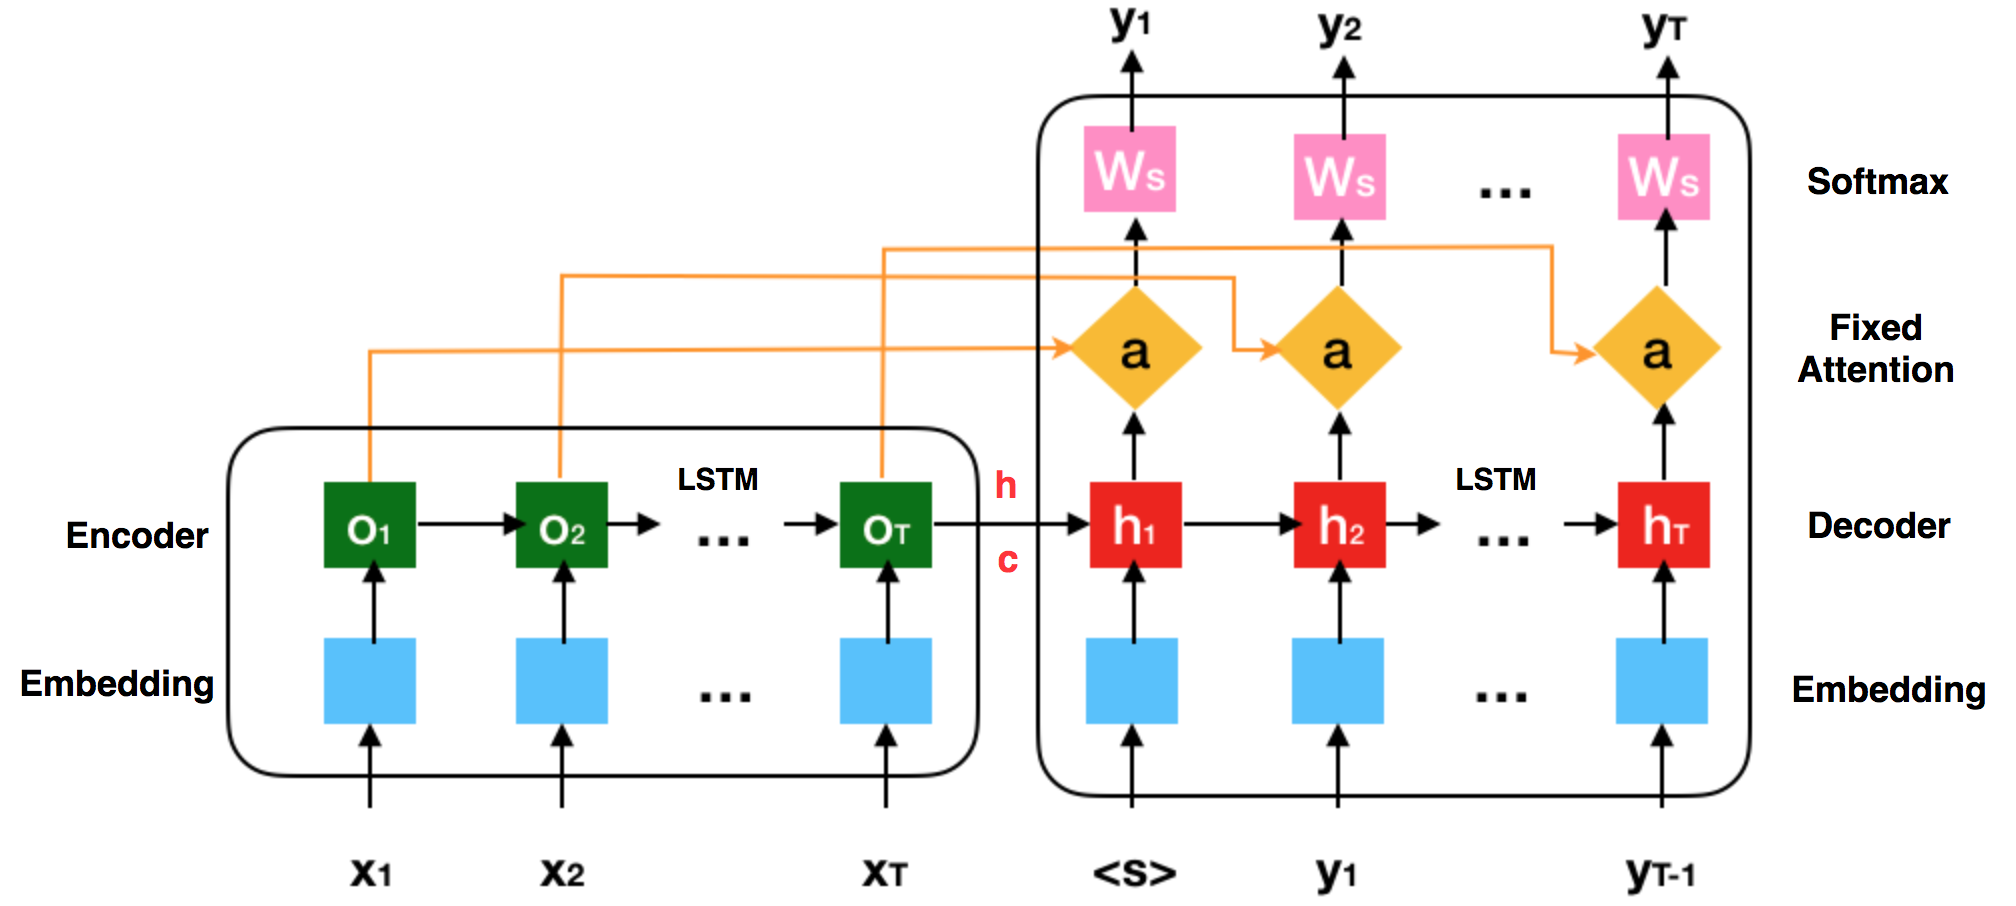
\includegraphics[width=1.0\linewidth]{archi.png}
\caption{Architecture of Seq2Seq model with fixed attention. The special token that denotes a beginning of a sentence is denoted as \texttt{<s>}. At each time step, the output $h^{dec}_t$ only looks back the corresponding input of the same time step $h^{enc}_t$ (denoted as $o_t$ in this figure).}
\label{fig:fig_architecture}
\end{figure}
%%%%%%%%%%%%%%%%%%%%%%%%%
As usual for text sequence, the encoder employs an RNN, which model output at each time step as: 
  \begin{equation}
	({h^{enc}_t}, {c^{enc}_t}) = RNN(h^{enc}_{t-1}, x_t)
  \end{equation}
where $h_i$ and $c_i$ denotes the hidden and cell state at time step $t$ respectively. Thus the encoder output $Z$ is the last hidden state $h_T$ and cell state $c_T$ as:
  \begin{equation} \label{eq:z}
      {Z} = ({h^{enc}_T}, {c^{enc}_T}) = RNN(h^{enc}_{T-1}, x^{enc}_T)	
  \end{equation}

\subsection{Seq2Seq Decoder}
As mentioned, the decoder will take encoder's output $Z$, and try to decode each token $\tilde{y_t}$ corresponding to $x_t$. It models the conditional probability: 
  \begin{equation}
      P(Y|Z,X) = \prod_{t=1}^{T} p(Y_t|{Z}, Y_1, ..., Y_{t-1})
  \end{equation}
with a note that $Y_0$ is the special token that denotes the start of a sentence. 

The Seq2Seq training target is to find the best translation sequence which is as close to the ground truth Y as possible, or formally:
  \begin{equation}
      \widehat{Y} = \operatorname*{arg\,max}_{Y} p(Y|Z, X) 
  \end{equation}
This is the phase where we employ the searching algorithm such as greedy search or beam search to decode each token. But essentially, the whole process consists of two phases. First is the RNN phase which is similar to the encoder: 
  \begin{equation}
      (h^{dec}_t, c^{dec}_t) = RNN(h^{dec}_{t-1}, y_t) \label{eq:rnn_dec}
  \end{equation}
where the initial hidden and cell state is set from the encoder by Equation \ref{eq:z}.

Similar to the encoder, the golden label sequence $Y$ is also first casted into an embedding $E_Y$, and then fed into the decoding RNN network. Note that, slightly different from the encoder, here it is $y_{t-1}$ that is fed into the RNN cell at step $t$ (hence the last label $y_{T}$ is not fed; the input sequence is $\{y_0, y_1, \dots, y_{T-1}\}$). For the initial input at step $t = 1$, we use a special token $y^* =$ \texttt{<BEG>} to denote the beginning of the label sequence.

The second phase is to convert the hidden state of tokens to the probability over the entire label space: 
  \begin{equation}
      p_{y_t} = softmax(W_{s} h^{dec}_t + b_{s}) \label{eq:pt}
  \end{equation}
where $W_{s}$ and $b_{s}$ are the shared weight and bias vector on top of the decoder's hidden layer. 

\subsection{Fixed Attention} \label{ssec:atten}
Attention model \cite{bahdanau2014neural,luong2015effective} is one of the useful tricks in training Seq2Seq models. The idea is, instead of using the RNN function as in Equation \ref{eq:rnn_dec} in which every output only depends on current input token and the previous hidden state, we augment this by giving it a chance to look back and calculate the similarity with each token in the encoder \textit{output} sequence. The similarity functions are varied in practice. 

Then the Equation \ref{eq:pt} for decoder output at step $t$ is transformed to: 
  \begin{equation}
      p_{y_t} = softmax(W_{s} \cdot attn(h^{dec}_t, h^{enc}) + b_{s}) \label{eq:pt_attn}
  \end{equation}
where the attention function is the re-weighted output \textit{w.r.t} the encoder output: 
  \begin{equation}
	  attn(h^{dec}_t, h^{enc}) = \sum^{T}_{i=1} h^{enc}_i * a_i \label{eq:attn}
  \end{equation}
and the activated weight function $a()$ is the softmax of similarity: 
  \begin{equation}
	  a = softmax(sim_1, sim_2, \dots, sim_T) \label{eq:a}
  \end{equation}
where the similarity function
  \begin{equation}
	sim_i = f_{sim}(h^{dec}_t, h^{enc}_i)
  \end{equation}
can be a as simple as a dot product $sim_i = h^{dec}_t \cdot h^{encT}_i $ \cite{luong2015effective} or a linear combination between them \cite{bahdanau2014neural}, as follow:  
  \begin{equation}
  	sim_i = (h^{dec}_t \cdot W^{dec} + h^{enc}_i \cdot W^{enc}) \cdot V
  \end{equation}
  
In our Tagging problems, we have a valuable prior that at every time step $t$: the output $h^{dec}_t$ is absolutely similar to $h^{enc}_t$, i.e. they have the same time step. Consequently, equation \ref{eq:a} will give the probability 1.0 to $sim_t$ and zero to the rest, leading to the change of equation \ref{eq:attn} into a simple form:
  \begin{equation}
	  attn(h^{dec}_t, h^{enc}) = h^{enc}_t
  \end{equation}

For implementation, we keep this "fixed" setting with Bahdanau attention, and so we only need to learn the parameters $W^{dec},W^{enc}, V$ before passing the decoder output into softmax in \ref{eq:pt_attn} for decoding. Figure \ref{fig:fig_architecture} illustrates our attention setting. And as a trick, we can concatenate $h^{dec}_t$ and $h^{enc}$ so that we only need learn only one matrix $W$ whose output dimension is the concatenated hidden sizes of both the encoder and decoder combined. 

\subsection{Seq2Seq Training}
Finally, to train the model, we use the canonical cross-entropy loss: 
  \begin{equation}
      \mathcal{L} = -log(P(Y|X)) = - \sum^T_{t=2} log(p_{y_t})
  \end{equation}
  
In detail, the traditional training which uses the teacher-forcing algorithm will feed the correct label $y_t$ to each time step $t$. But this oftentimes leads to an unwanted behavior where an error in will propagate severely at test time, when the model has no idea about the gold labels. By using this training scheme, the model is not able to learn about how to handle a wrong prediction properly. 

One popular method is to employ a schedule where teacher-forcing is used at a random chance at each step, and the other chance is to feed the predicted $\tilde{y_t}$ instead of the gold label $y_t$ and let the model learn to penalize and correct wrong predictions appropriately. 

% \subsection{Training-time decoding}

% In training time, the decoder receives the last hidden and cell states from the encoder as the initial hidden and cell states, respectively:
% \begin{align}
% 	h_0 &= \overrightarrow{h}_{T_x}, \\
% 	%
% 	c_0 &= \overrightarrow{c}_{T_x}.
% \end{align}
% The golden label sequence $Y = \{y_1, y_2, \dots, y_{T_y}\}$ is also first casted into an embedding created by the target-space embedding layer $E^y$, and then fed into the decoding LSTM network. Note that, slightly different from the encoder, here it is $y_{t-1}$ that is fed into the LSTM cell at step $t$ (hence actually the last label $y_{T_y}$ is not fed as the input of the decoder; the input sequence is $\{y_0, y_1, \dots, y_{T_y - 1}\}$). For the initial input at step $t = 1$, we use an universal $y_0 = y_0^*$ to denote the beginning of the label sequence.

% The hidden states $h_t$ is then fed into a linear layer to produce the score vector $s_t$, where each element of $s_t$ is the score for each of the possible labels at step $t$:
% \begin{align}
% 	s_t = W_s h_t + b_s.
% \end{align}
% We then take the softmax over the score vector $s_t$ to obtain the probabilities of all possible labels at step $t$,
% \begin{align}
% 	\label{eq:pt} p_t = \textrm{softmax}(s_t).
% \end{align}

% The loss at step $t$ is the cross entropy between the prediction $p_t$ and the golden label $y_t$,
% \begin{align}
% 	L_t = -\log (p_t)_{y_t}.
% \end{align}
% The total loss for this sequence instance is the average of the loss over the steps,
% \begin{align}
% 	L = \frac{1}{T_y} \sum_t L_t.
% \end{align}
% We take average in hope to remove the bias introduced by the length of the sequence.



\subsection{Test-time decoding}

In test time, as in training time, the decoder receives the last hidden and cell states from the encoder as initial states. The initial input at step $t = 1$ is also the universal special token $y^* =$ \texttt{<BEG>} or \texttt{<s>}. But, different from training time, the inputs at time steps $t = 2, \dots, T - 1$ depend on the predicted label at the previous step. Roughly speaking, we would $replace$ the input $y_{t-1}$ by $\hat{y}_{t-1}$ at test time. The exact way to do so is determined by the decoding algorithm.

Note that, similar to the case of attention, we can have a much simpler decoding algorithm since we know beforehand the (equal) length of output given an input, so we will not take care of the difficulty of handling stopping criteria for this phase.  

\subsubsection{Greedy Search}
Greedy decoding at test time is to greedily pick the best prediction (with the highest probability) at each time step as the only selection criterion. 

Formally, at step $t=1$, we compute $p_{y_1}$ using \eqref{eq:pt}, and pick the token $\hat{y}_1$ that has the highest probability $p_1 = max(p_{y_1})$ as our predicted label. 

Next, we keep an accumulated probability $P_t$ initialized as $P_1 = p_1$. At step $t = 2, 3, \dots, T_y$, after computing $p_t$, we first compute the accumulated probability $P_t = p_t * P_{t-1} = \prod_{i=1}^{t-1} p_i$, and then pick the label $\hat{y}_t$ which has the highest probability $P_t$ as our predicted label at step $t$. 

In practice, we consider $log(P_t)$ instead of $P_t$ to prevent the common numeric underflow issue. 

\subsubsection{Hard Beam Search}
Extended from greedy search, hard beam search, although more architecturally and hence computationally expensive, is more widely, and traditionally used \cite{seq2seq_2014} for it is able to prevent the label bias problem in Seq2Seq models. It is also known as \textit{TopK} searching algorithm because at every step, instead of considering the maximum value, it always maintains a window of size $K$ for the best $K$ options. For this reason, greedy search is just its special case where $K=1$. 

For example, at step $t=1$, instead of picking the only $\hat{y}_1$, we keep the $K$ best labels $\{ \hat{y}^{(1)}_{1}, \hat{y}^{(1)}_{2}, \dots, \hat{y}^{(1)}_{K} \}$. Note that we need a tracking table mapping the words in vocabulary to those labels. Similar to greedy search, we keep the accumulated probabilities $\{ P_1, P_2, ..., P_K \}$, which are initialized as 
$\{ p(y^{(1)}_{1}), p(y^{(1)}_{2}), \dots, p(y^{(1)}_{K}) \}$. We start to build a tree with K branches. 

In detail, later at time step $t$, we have $K$ options of inputs $\{ y^{(t)}_k\}^{k=1}_K$, and for each input $y^{(t-1)}_{k}$, we also calculate K best probabilities $\{ p({y}^{(t)}_{k1}), p({y}^{(t)}_{k2}), \dots, p({y}^{(t)}_{kK}) \}$. Note that this time step, we still only keep $K$ branches in total, i.e. we keep only the best global cases across all beams (also based on the accumulated log probabilities) along with recording the mapped label associated with that probability. Finally, the highest accumulated sum-log will be chosen and the predicted label sequence is pulled out by backtracking the mapping table. 

Compared with greedy search, hard beam search with fixed beam size trades processing time with the accuracy since best scoring sequence will eventually be captured as the beam size grows. However, it always process $B * |V_{label}|$ tokens where $B$ is beam size at each time step, which consumes not only a a large amount of time but memory as well. 


%%%%%%%%%%%%%%%%%%%%%%%%%%%%%%%%%
%         MODEL              
%%%%%%%%%%%%%%%%%%%%%%%%%%%%%%%%%
\section{Adaptive Beam Search by Heuristic Pruning and Growing}
\label{sec:Heuristic}

To increase the search efficiency as well as the optimality of the resulting sequence, we propose the heuristic rules to prune or grow the beam size of the search tree space during the test-time decoding. The intuition behind the design is that, if we predict that some branches are much more probable than the rest of the branches, it might be reasonable to skip searching through the less probable branches. Furthermore, unlike fixing the beam size, we should also include as many beams as possible if they are comparably probable candidates at each time step.

In this work, we adopt the novel approach that we only incrementally increase or decrease the beam size during the search process. Such design choice facilitates the comparison between the performance of the heuristic rules and the reinforcement learning agent we will be discussing later in Section ~\ref{sec:RL}.

In detail, consider that at time step $t$ of the decoding, there are $B_{t-1}$ inputs, $\hat{y}_{t-1}^{(b)}$, $b = 1, \dots, B_{t-1}$, from the $B_{t-1}$ previous step of the decoder output. By decoding these $B_{t-1}$ inputs, we obtain $B_{t-1} \times |V^y|$ probability predictions for the $|V^y|$ possible targets in $B_{t-1}$ beams. We sort the $B_{t-1} \times |V^y|$ probabilities into a sorted list $\{ P_1, \dots, P_{B_{t-1} |V^y|} \}$, with $P_1$ being the highest probability. We then pick the first $B_t$ elements from the list to form the new beam produced by this decoding step, with the corresponding target words $\{ \hat{y}_{t}^{(1)}, \dots, \hat{y}_{t}^{(B_t)} \}$. In the standard beam search where the beam size is kept fixed, we have $B_t = B_{t-1}$ at each step.

We propose the following heuristic rules to dynamically change the beam size at each step.
\begin{itemize}
\item If $\displaystyle{\frac{\prod'_t P_{B_{t-1}}}{\prod'_t P_1}} \leq r^{\textrm{sen}}_{\textrm{low}}$ or $\displaystyle{\frac{P_{B_{t-1}}}{P_1}} \leq r^{\textrm{word}}_{\textrm{low}}$, then decrease the beam size: $B_t = B_{t-1} - 1$.
\item If $\displaystyle{\frac{\prod'_t P_{B_{t-1}}}{\prod'_t P_1}} > r^{\textrm{sen}}_{\textrm{low}}$ or $\displaystyle{\frac{P_{B_{t-1}}}{P_1}} > r^{\textrm{word}}_{\textrm{low}}$, then increase the beam size: $B_t = B_{t-1} + 1$.
\end{itemize}
The primed summation $\prod'_t$ notation is used to indicate that the product is taken over the path of this beam from $t = 1$ to this step. For example, $\prod'_t P_1$ denotes the cumulative probability for the sequence of the top-1 beam. The thresholds  $r^{\textrm{sen}}_{\textrm{low}}$ and $ r^{\textrm{word}}_{\textrm{low}}$ are chosen heuristically. Note that to avoid numerical underflow, we work in the logarithmic space as we implement the rules.

%HERE...





\section{Adaptive Beam Search by Reinforcement Learning}
\label{sec:RL}

Using the heuristic rules to prune or grow the beam size has a downside that the thresholds of pruning or growing (the parameters $r^{\textrm{sen}}_{\textrm{low}}$ and $r^{\textrm{word}}_{\textrm{low}}$ in our case) are set by hand, which may require some tuning to find the suitable values. Moreover, the thresholds suitable for one task is generally different from those for another task, so additional human labor is needed to identify the suitable thresholds for each new task.

To overcome the shortcoming of the heuristic algorithm, we propose the second approach to perform the adaptive beam search by introducing an ``agent'' to learn when to increase or decrease the beam size, using reinfor

\subsection{Reinforcement learning environment}
Particularly, we consider the scenario that there is an agent observing the predicted probability distribution at each step of the decoder output, and then determines to take an action among three possible actions towards the beam size, which are \textit{\{decrease, keep, increase \}}.

%HERE...

\begin{figure}[ht]
\centering
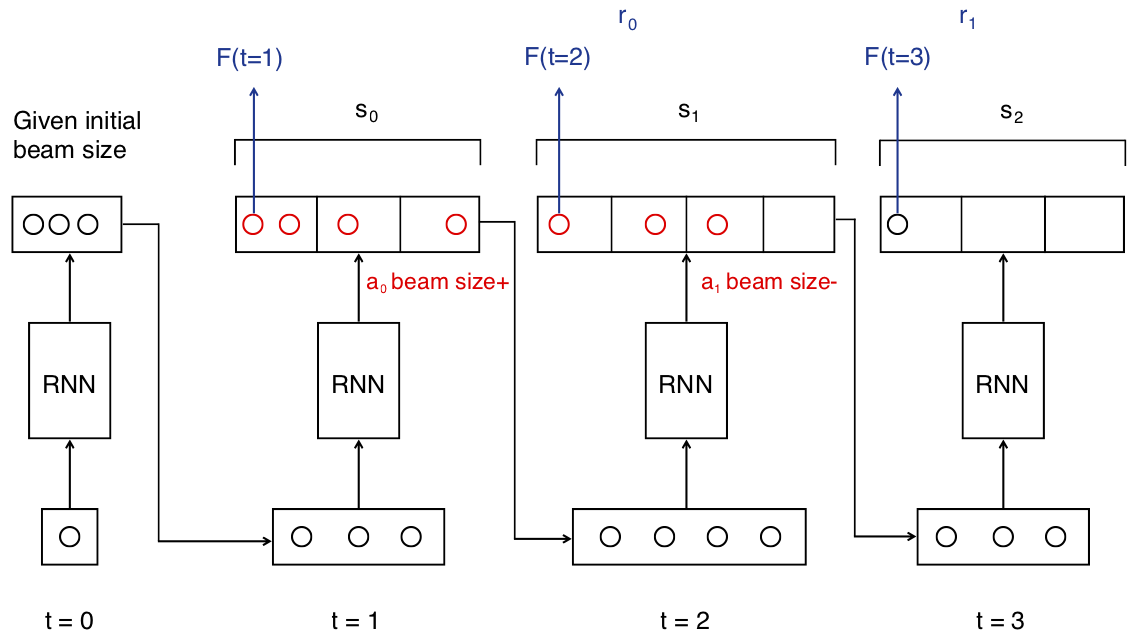
\includegraphics[width=1.0\linewidth]{adapt.png}
\caption{Demonstration of how agent learns to adapt beam size for decoding. At $t=1$, it learns to increase the beam size from 3 to 4. At $t=2$, it reduce the beam size back to 3.}
\label{fig:adaptve}
\end{figure}

For the most important part is the reward, we combine 3 different numbers given a timestep $t$: 
\begin{itemize}
	\item Cumulative log probability of the beams from timestep $0$. This criterion is traditionally used in beam search for Seq2Seq model. 
    \item Current log probability of top words in the beams. 
    \item Current beam size 
\end{itemize}

For implementation, we flatten out those numbers and thus obtain a vector of length $2 * \text{max\_beam\_size} + 1$. 
\subsection{Training Decoder with Asynchronous Advantage Actor-Critic Method}


\begin{figure}[ht]
\centering
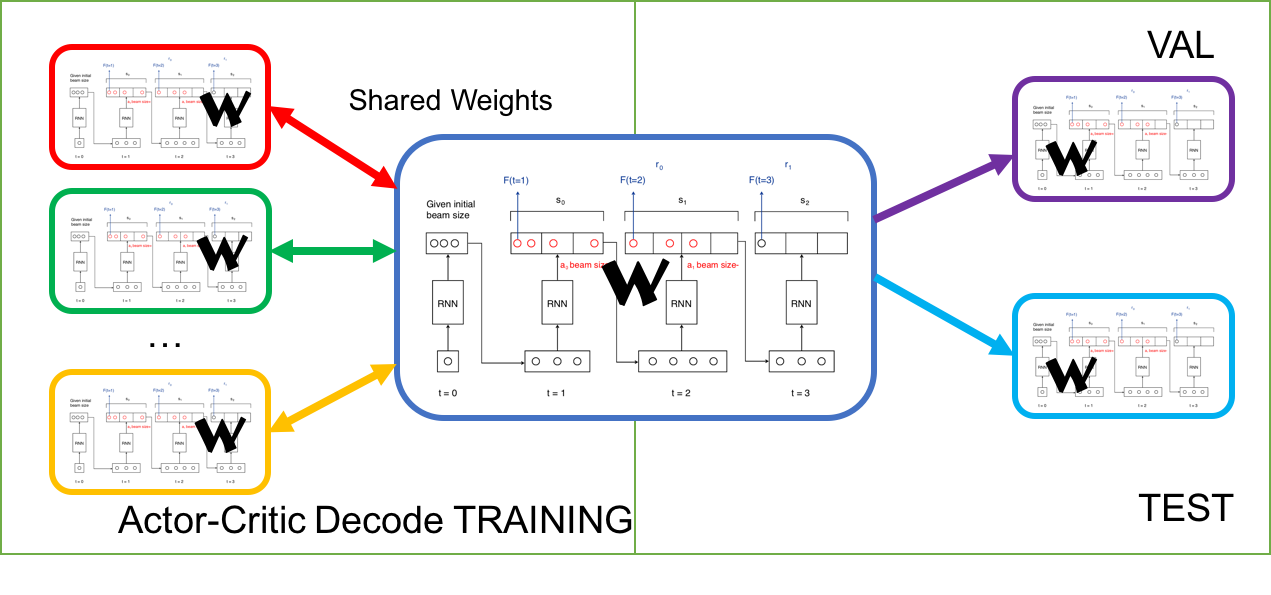
\includegraphics[width=1.0\linewidth]{a3c.png}
\caption{A3C training with multiple training agents which are all able to update the parameters to the shared model. For validation and testing, these parameters are copied to the respective validation and test agents.}
\label{fig:a3c}
\end{figure}

Actor-Critic RL \cite{sutton1998reinforcement} is known to be a popular method to effectively training a RL agent using REINFORCE \cite{williams1992simple} because it allows to end the episode early. But we choose Asynchronous Advantage Actor-Critic (A3C) \cite{mnih2016asynchronous} to implement our algorithm for simplicity (compared with other state-of-the-art methods), ability to resolve high variance and high sample complexity in training of Actor-Critic and parallelism which helps speed up the training. 

Our A3C architecture is shown in Figure \ref{fig:a3c}. From the environment defined above, we use a shared model and initialize many training agents which share the same optimizer as well, to asynchronously update the model policy network during training. Each episode stands for each sentence containing the tagging task for each token in the sentence. 

\section{Experiments}

Our implementation\footnote{The Github repository is accessible at: https://github.com/ShuxinLin/nn4nlp\_project/.} is built based on PyTorch \cite{paszke2017automatic}. We conducted all experiments on AWS EC2 as well as private computers. As it is discussed in Section \ref{ssec:model}, the current Seq2Seq model is built on the encoder-decoder architecture. For encoder, we use one-layer bi-directional LSTM, and for the decoder we use one-layer single-directional LSTM with a fixed attention mechanism. We perform the training using mini-batch stochastic gradient descent with Adam optimizer and use different beam search strategies in testing time. The task we are trying to solve is two common natural language processing tasks, the named entity recognition (NER) and CCG Supertagging.

\subsection{Datasets}
In order to make our experimental results comparable to the baseline \cite{goyal2017continuous}, we use the same datasets as well as evaluation metrics. 

For named entity recognition, we use the data of CONLL-2003 shared task \cite{tjongkimsang2003conll} for German language. The data consists of three files per language: one training file and two test files, testa and testb. We use testa as the development data, testb as the final test data.  The label/entity has 9 possible values: 8 NER tags and a tag denoting the end of the sentence (EOS). Due to the extremely skewed label distribution towards the default label ($O$), the widely-used evaluation metrics for this dataset is F score.

 For CCG Supertagging task, we use the data of CCGbank corpus \cite{hockenmaier2007ccgbank} and its provided splits for train, development, and test data. The label has 1321 possible values: 1320 CCG derivation grammar tags and a tag denoting the end of the sentence (EOS). In this task, accuracy of correct predictions is measured.

We perform very minor preprocessing on the data by creating and indexing the vocabulary of each datasets. Given the vocabulary of input words, we construct pre-trained word embedding matrix using GloVe for English and provided word embedding \cite{goyal2017continuous} for German. 
As can be noticed above, CCG Supertagging task have larger label size (search space) than NER task. Thus it leads to the fact that CCG supertagging task is more appropriate for measuring the efficacy of the proposed dynamic beam search methods.  



\subsection{Results and Analysis}

The results of the heuristic pruning and growing adaptive beam search on the NER and CCG datasets are shown in Table \ref{tab:NERHeuristic} and \ref{tab:CCGHeuristic}, respectively. From the results of NER dataset, we observe that using heuristic adaptive beam search effectively reduces the search space and the search time, while not sacrificing the F-score. In the case of initial beam size 9, the total number of beams explored during decoding in the adaptive case is only $42\%$ of that in the case of fixed beam size, while the F-score using adaptive search only decreases by less than $0.1\%$; measured in time, the decoding time is reduced to $52\%$ when using adaptive method. Note that in the NER dataset, greedy search gives higher F-score than the beam search methods do. This is consistent with the results from the baseline.


\begin{table*}[ht]
\centering
\caption{Heuristic pruning and growing rules results. NER.}
\label{tab:NERHeuristic}
\begin{tabular}{lcccccccc}
\toprule
& Greedy & Beam 3 & Beam 3 & Beam 6 & Beam 6 & Beam 9 & Beam 9 & Soft Beam \\
& & & Adaptive & & Adaptive & & Adaptive & \\
\midrule
F-score & 58.09 & 57.69 & 57.71 & 57.76 & 57.71 & 57.76 & 57.71 & \\
Total beam \# & 48,571 & 145,713 & 92,727 & 291,426 & 126,759 & 437,139 & 182,785 & \\
Avg.~beam \# & 1 & 3 & 1.95 & 6 & 3.16 & 9 & 4.86 & \\
Time (sec) & 22 & 76 & 61 & 132 & 73 & 178 & 92 & \\
\midrule
Goyal 2017 & 54.92 & 51.34 & & & & & & 56.38 \\
F-score \\
\bottomrule
\end{tabular}
\end{table*}



\begin{table*}[ht]
\centering
\caption{Heuristic pruning and growing rules results. CCG.}
\label{tab:CCGHeuristic}
\begin{tabular}{lccccccc}
\toprule
& Greedy & Beam 1 & Beam 2 & Beam 2 & Beam 3 & Beam 3 & Soft Beam \\
& & Adaptive & & Adaptive & & Adaptive & \\
\midrule
Accuracy & 90.50 & 90.62 & 90.60 & 90.62 & 90.62 & 90.62 &  \\
Total beam \# & 52,964 & 93,403 & 105,928 & 98,100 & 158,892 & 103,875 &  \\
Avg.~beam \# & 1 & 1.61 & 2 & 1.72 & 3 & 1.87 &  \\
Time (sec) & 22 & 87 & 92 & 130 & 184 & 141 &  \\
\midrule
Goyal 2017 & 80.35 &  & & & 82.42 & & 82.00 \\
Accuracy \\
\bottomrule
\end{tabular}
\end{table*}


The performance of the adaptive search is better on the CCG dataset. We observe the following:
\begin{enumerate}
\item By starting with initial beam size of 1, and allow the beam size to be adaptively changed in the following steps during decoding, we obtain higher accuracy than the greedy search (always keep beam size 1) does.
\item Using fixed beam size, one needs to use beam size 3 to obtain the same accuracy achieved by the adaptive beam search with initial beam size 1, while the latter only needs to explore about $59\%$ of the beam number, and spends only $47\%$ of the time.
\item The F-scores obtained by using different initial beam size for the adaptive search are stable (actually the same value in this experiment), and the total number of beams explored by using initial beam size 3 increases by only $11\%$ compared to that by using initial beam size 1.
\end{enumerate}





The results of the adaptive beam search using the reinforcement learning agent on the NER dataset is shown in Table \ref{tab:NERRL}.


\begin{table}
\centering
\caption{Reinforcement learning results. NER.}
\label{tab:NERRL}
\begin{tabular}{lccc}
\toprule
& Beam 3 & Beam 6 & Beam 9 \\
\midrule
F-score & 57.66 & 57.61 & 57.52 \\
Avg.~beam \# & 1.17 & 2.00 & 3.06 \\
\bottomrule
\end{tabular}
\end{table}










% The data consists of three files per language: one training file and two test files, testa and testb. We use testa as the development data, testb as the final test data. In the current development phase, only the train data and the development data are used for finding good parameters for the seq2seq model.

% We perform minimum preprocessing on the data, since the best performance is not our ultimate goal of this project, but the effectiveness of the improvement we propose. The label has 9 possible values: 8 NER tags and an additional tag denoting the beginning of the sentence ($\langle$BEG$\rangle$).


% \subsection{Design Improvements over Assignment 1 and Results}



% \subsubsection{New data batching scheme}
% In the previous impelementation, mini batches of data inputs were fixed-sized sentences, so that paddings were appended the original sentences which introduces irrelevant information. Now we impelement the scheme to support variable-sized batches. In this case, the paddings are not needed. Moreover, we add data shuffling at the beginning of each epoch. This avoids the order of incoming sequences have impact on the results.

% \subsubsection{Initialized by pre-trained word embeddings}
% We initialized word embeddings by pretrained weights as discussed in the Section 3.2. The word embedding dimension of Word2Vec, GloVe and fastText is 300 for each word; while the dimension of the version provided by \citet{goyal2018continuous} is 64. One commmon issue of pretrained word embedding model is Out-of-Vocabulary issue, i.e. some of words in our vocabulary are not in the vocabulary of pretrained word embeddings. For English datasets, GloVe model has larger vocabulary set, and mismatched cases using GloVe are much less than using Word2Vec. Thus GloVe is our choice. For German datasets, we use the version provided by \citet{goyal2018continuous} since the word embedding dimension is smaller.

% The vectorized word embeddings are pre-computed and saved as the Numpy array format of shape (vocabulary\_size, embedding\_dimension). The results are shown in Table \ref{embed}. The experiments set up in the same configureation except whether use the pretrained word embeddings or not. From the table, we can see that although the accuracy does not make differences, the F score of train data using pre-trained word embeddings significantly improves.

% Please add the following required packages to your document preamble:
% \usepackage{booktabs}
% \begin{table}[ht]
% \centering
% \caption{After 30 epoches, the results of models on train data with and without pre-trained word embeddings. The model without pre-trained word embeddings creates word embeddings by random initialization. }
% \label{embed}
% \begin{tabular}{@{}llll@{}}
% \toprule
% Model                     & CE loss  & Accuracy & F-score \\ \midrule
% w/ pre-trained          & 0.1377 & 94.21\%  & 46.84   \\
% w/o pre-trained & 0.1927 & 92.76\%  & 30.82   \\ \bottomrule
% \end{tabular}
% \end{table}

% \subsubsection{Using bi-directional LSTM in encoder}

% 	In assignment 1 we use single directional LSTM as the encoder. In this assignment, we extend the encoder to bi-directional LSTM network. To feed the last hidden state and cell state into the encoder, we use a linear layer (without bias term) to combine the two $R^h$ vectors into a single $R^h$ one. The very linear layer for the hidden state is later used again in the attention mechanism to prepare the ``annotation'' of the encoded sequence.

% \subsubsection{Beam search implementation}

% 	We implemented beam search for test-time decoding in this assignment. The beam search implementation is compatible with the attention mechanism. We handled the back-tracking of the beam search process, so that the function will return the optimal output sequence found with given constant beam size, as well as the predicted score distribution and attention coefficient matrix of this sequence.
    
%     We compare the cross-entropy loss function and the F-score of experiments with and without beam search. For beam search, we use beam size of 3 and 10. We train our model for 50 epochs. The resulting F-score is listed in Table \ref{tab:beam}. The training curve is given in Figure \ref{fig:no_attn_losses_fscore}.

% ========================================================================================================
% ========================================================================================================

% \begin{table}[ht]
% \centering
% \caption{The training and validation F-score of experiments with and without beam search. Beam sizes are 3 and 10.}
% \label{tab:beam}
% \begin{tabular}{lrr}
% \toprule
%                   & F-score  & F-score    \\
%                   & (train)  & (val)    \\ \midrule
% Greedy            & 52.81            & 2.88                    \\
% Beam search (size 3)   & 43.47            & 4.05                    \\
% Beam search (size 10)  & 25.60            & 3.35                    \\ \bottomrule
% \end{tabular}
% \end{table}

% ========================================================================================================
% ========================================================================================================
% \begin{table*}[ht]
% \centering
% \begin{tabular}{cc}
% \end{tabular}
% \begin{subfigure}{0.4\textwidth}\centering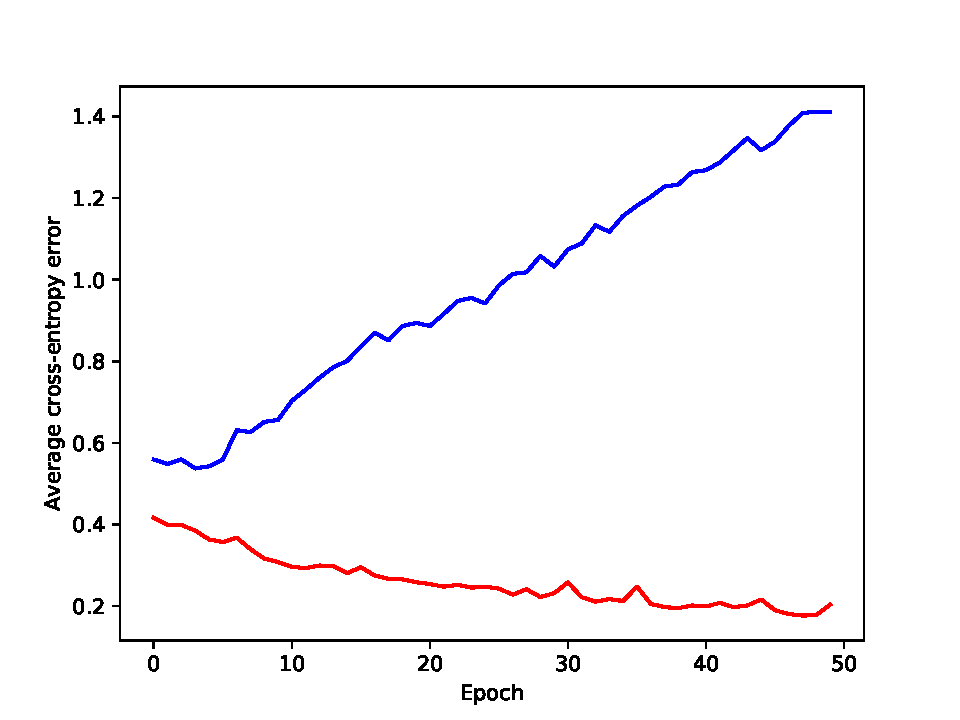
\includegraphics[width=0.7\columnwidth]{fig_lrn_0p001_loss.pdf}\caption{Greedy Search Decoding Loss}\end{subfigure} %\&
% \begin{subfigure}{0.4\textwidth}\centering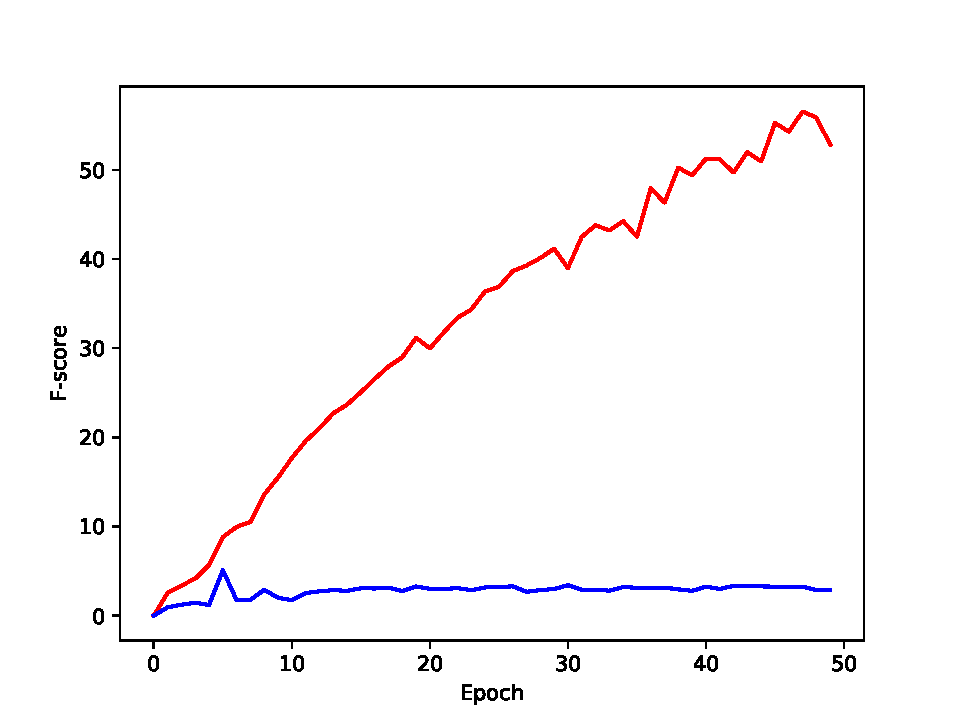
\includegraphics[width=0.7\columnwidth]{fig_lrn_0p001_f.pdf}\caption{Greedy Search Decoding F-Score}\end{subfigure} \\
% %%%%%%%%%
% \begin{subfigure}{0.4\textwidth}\centering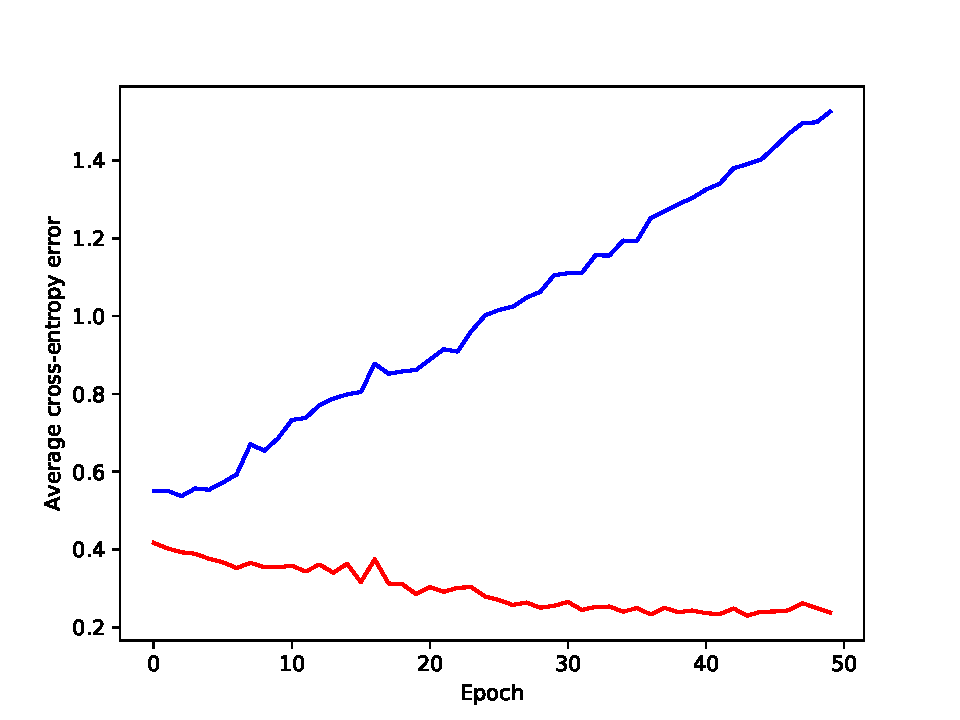
\includegraphics[width=0.7\columnwidth]{fig_lrn_0p001_beam_3_loss.pdf}\caption{Beam Search Decoding Loss}\end{subfigure} %\&
% \begin{subfigure}{0.4\textwidth}\centering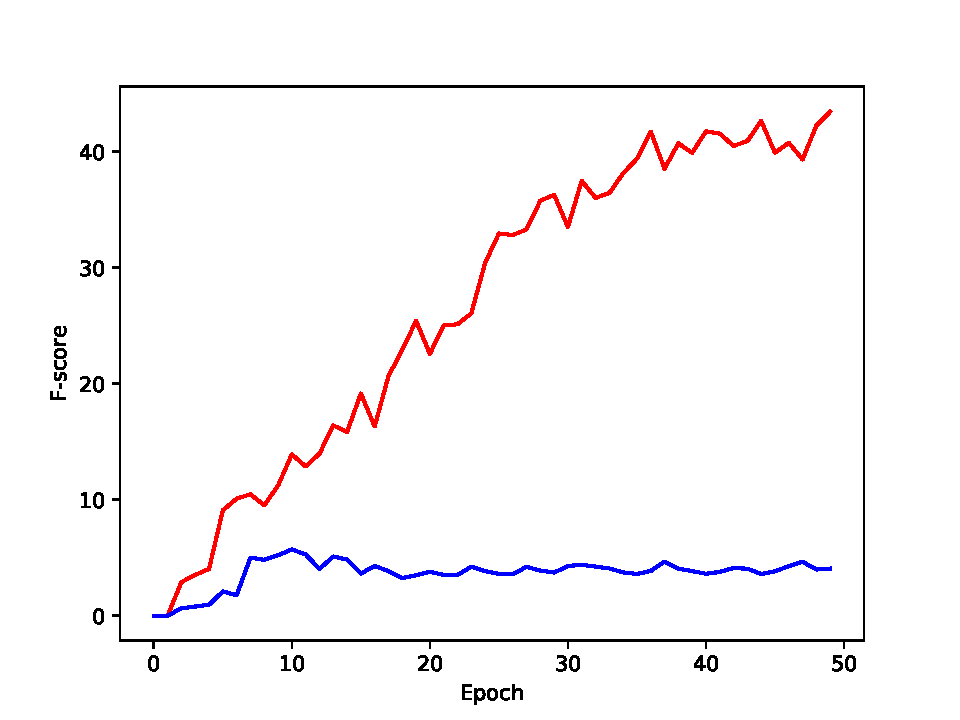
\includegraphics[width=0.7\columnwidth]{fig_lrn_0p001_beam_3_f.pdf}\caption{Beam Search Decoding F-Score}\end{subfigure} \\
% %%%%%%%%%
% \begin{subfigure}{0.4\textwidth}\centering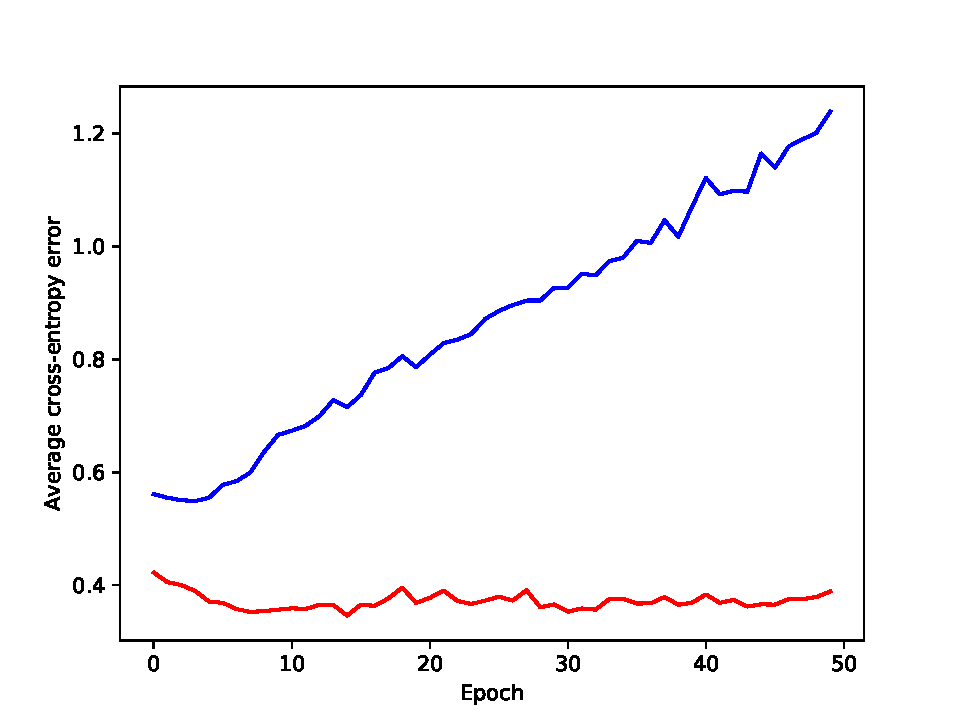
\includegraphics[width=0.7\columnwidth]{fig_lrn_0p001_beam_10_loss.pdf}\caption{Beam Search Decoding Loss}\end{subfigure} %\&
% \begin{subfigure}{0.4\textwidth}\centering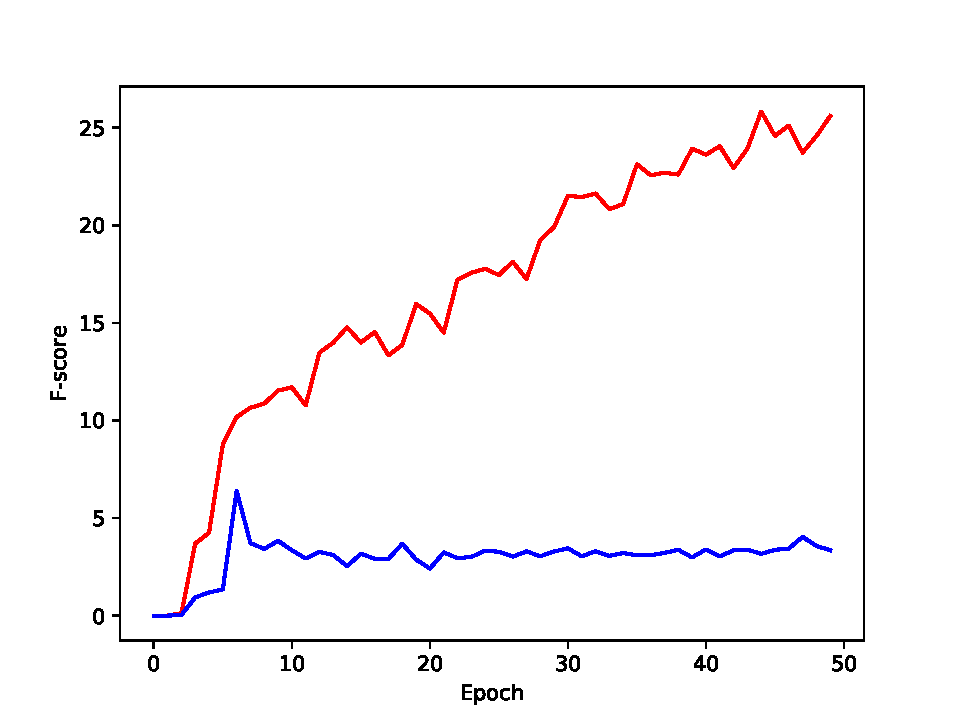
\includegraphics[width=0.7\columnwidth]{fig_lrn_0p001_beam_10_f.pdf}\caption{Beam Search Decoding F-Score}\end{subfigure} \\
% \captionof{figure}[]{The cross-entropy losses and F-scores of greedy and beam search decoding \textbf{without} attention. Red curve is training set, and blue curve is validation set. Learning rate is 0.001. For beam search, the beam size used in (c) and (d) is 3, and the beam size in (e) and (f) is 10.}
% \label{fig:no_attn_losses_fscore}
% \end{table*}
% ========================================================================================================
% ========================================================================================================

% \begin{figure}[ht]
% \centering
% 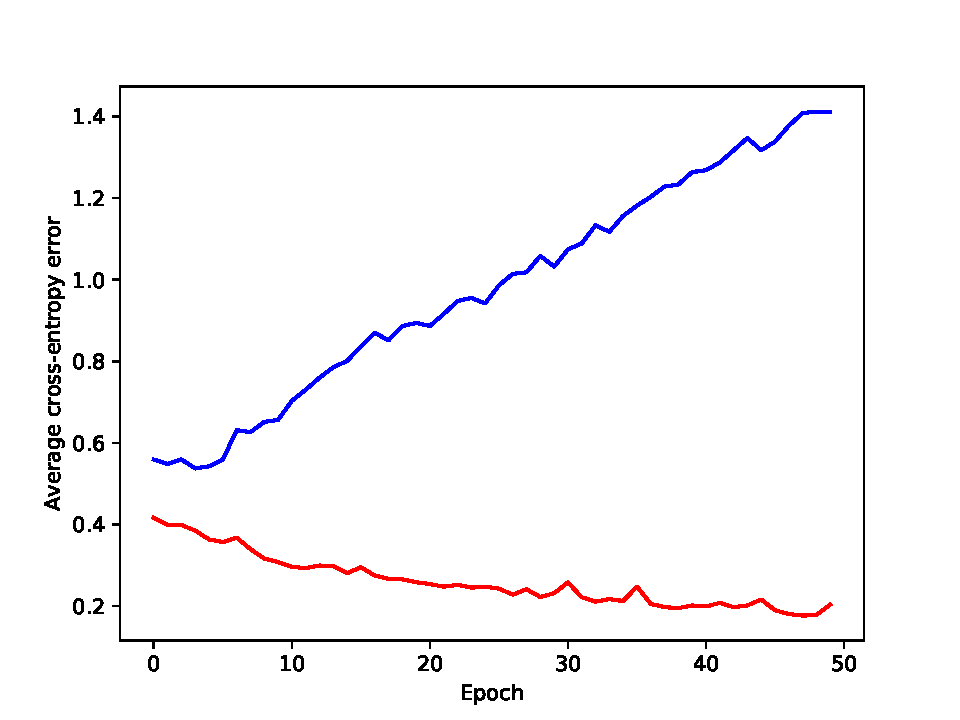
\includegraphics[width=0.8\linewidth]{fig_lrn_0p001_loss.pdf}
% \caption{The cross-entropy loss with greedy decoding. Red curve is training set, and blue curve is validation set. Learning rate is 0.001. No attention.}
% \label{fig:fig_lrn_0p001_loss}
% \end{figure}

% \begin{figure}[ht]
% \centering
% 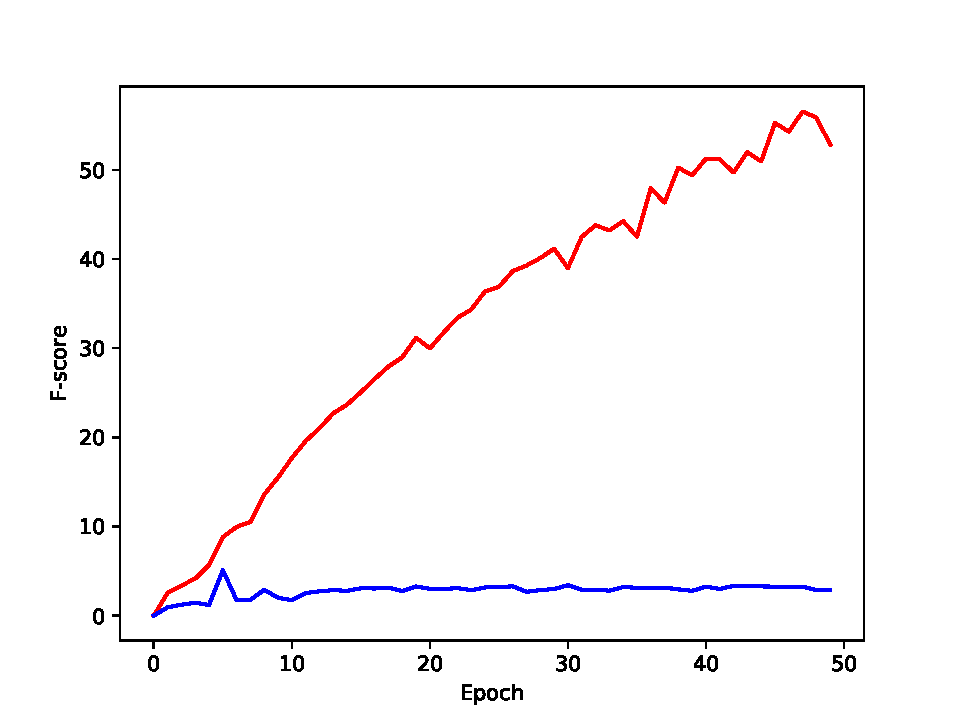
\includegraphics[width=0.8\linewidth]{fig_lrn_0p001_f.pdf}
% \caption{The F-score with greedy decoding. Red curve is training set, and blue curve is validation set. Learning rate is 0.001. No attention.}
% \label{fig:fig_lrn_0p001_f}
% \end{figure}

% \begin{figure}[ht]
% \centering
% 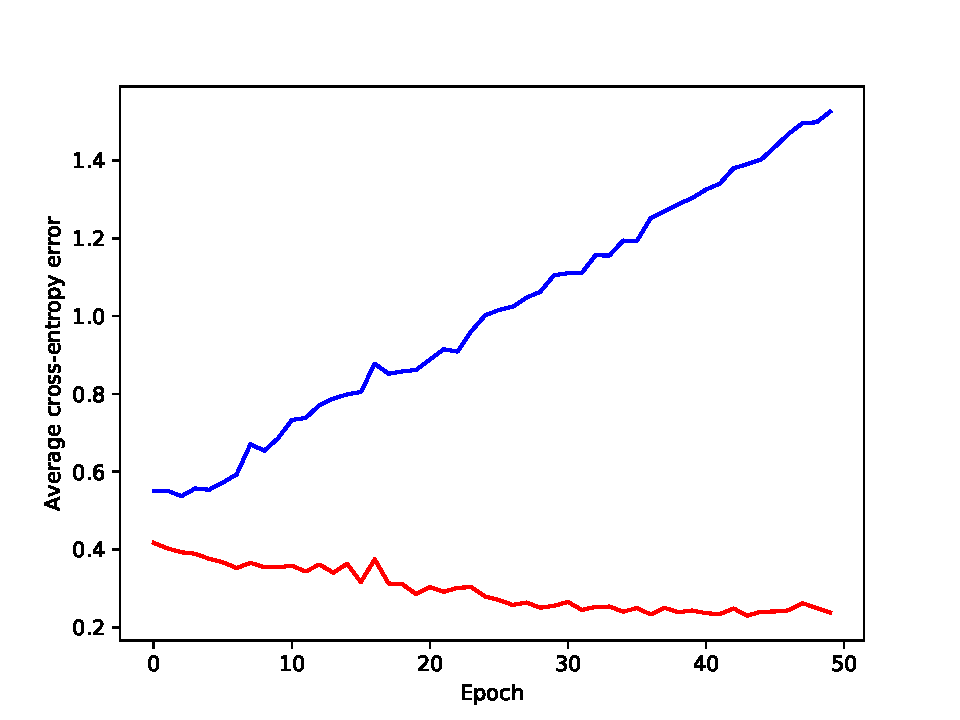
\includegraphics[width=0.8\linewidth]{fig_lrn_0p001_beam_3_loss.pdf}
% \caption{The cross-entropy loss with beam search decoding. Beam size is 3. Red curve is training set, and blue curve is validation set. Learning rate is 0.001. No attention.}
% \label{fig:fig_lrn_0p001_beam_3_loss}
% \end{figure}

% \begin{figure}[ht]
% \centering
% 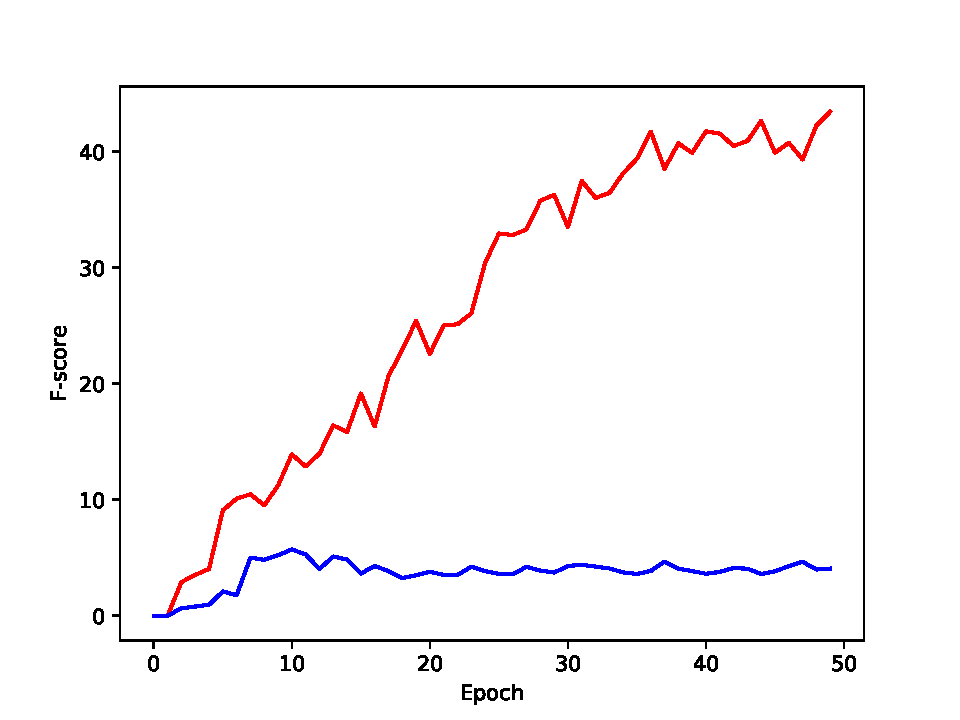
\includegraphics[width=0.8\linewidth]{fig_lrn_0p001_beam_3_f.pdf}
% \caption{The F-score with greedy decoding. Beam size is 3. Red curve is training set, and blue curve is validation set. Learning rate is 0.001. No attention.}
% \label{fig:fig_lrn_0p001_beam_3_f}
% \end{figure}


% \subsubsection{Attention implementation}

% 	We implemented a general class for attention mechanism. It currently focuses on fixed attention, which is used in our NER experiments, but it can be readily extended to support other attention mechanism such as Bahdanau attention. In our implementation for fixed attention, the attention module takes in the sequence of hidden state vectors from the bi-directional LSTM encoder, and the hidden state vector of the decoder at some current time step, as well as a ``combiner'' layer that is used to combine the two directions of the hidden vectors (each of dimension of $R^h$) of encoder into a single vector of dimension $R^h$. This single vector is the so-called ``annotation'' vector. This combiner used in our experiments is the same as the layer we used to transform the last two hidden state vectors (from two directions) of the encoder into one initial hidden state as the input of the decoder. We do not include bias term in the combiner. The result of adding attention is shown in Table \ref{tab:atten}.

% \begin{table}[ht]
% \centering
% \caption{The training and validation F-score of experiments with and without attention. For beam search, the beam size is 3.}
% \label{tab:atten}
% \begin{tabular}{lrr}
% \toprule
%                   & F-score  & F-score    \\
%                   & (train)  & (val)    \\ \midrule
% Greedy          & 52.81            & 2.88                    \\
% Greedy + Atten  & 96.60            & 3.14                    \\ 
% Beam              & 43.47            & 4.05                    \\
% Beam + Atten          & 78.78            & 3.87               \\ \bottomrule
% \end{tabular}
% \end{table}

% ========================================================================================================
% ========================================================================================================
% \begin{table*}[ht]
% \centering
% \begin{tabular}{cc}
% \end{tabular}
% \begin{subfigure}{0.4\textwidth}\centering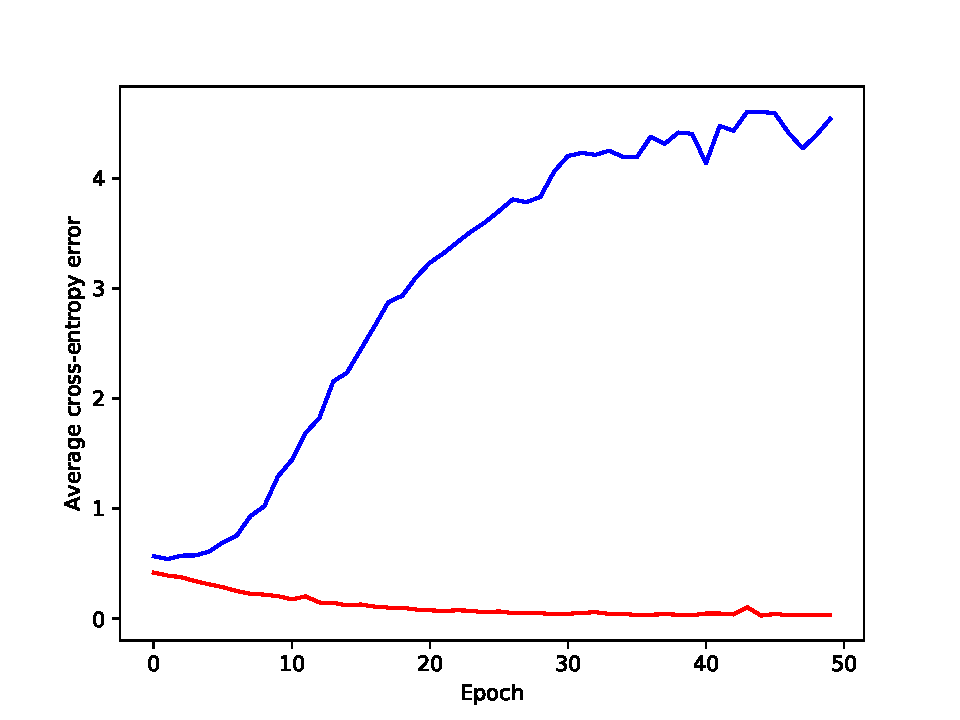
\includegraphics[width=0.7\columnwidth]{fig_lrn_0p001_atten_loss.pdf}\caption{Greedy Search Decoding Loss}\end{subfigure} %\&
% \begin{subfigure}{0.4\textwidth}\centering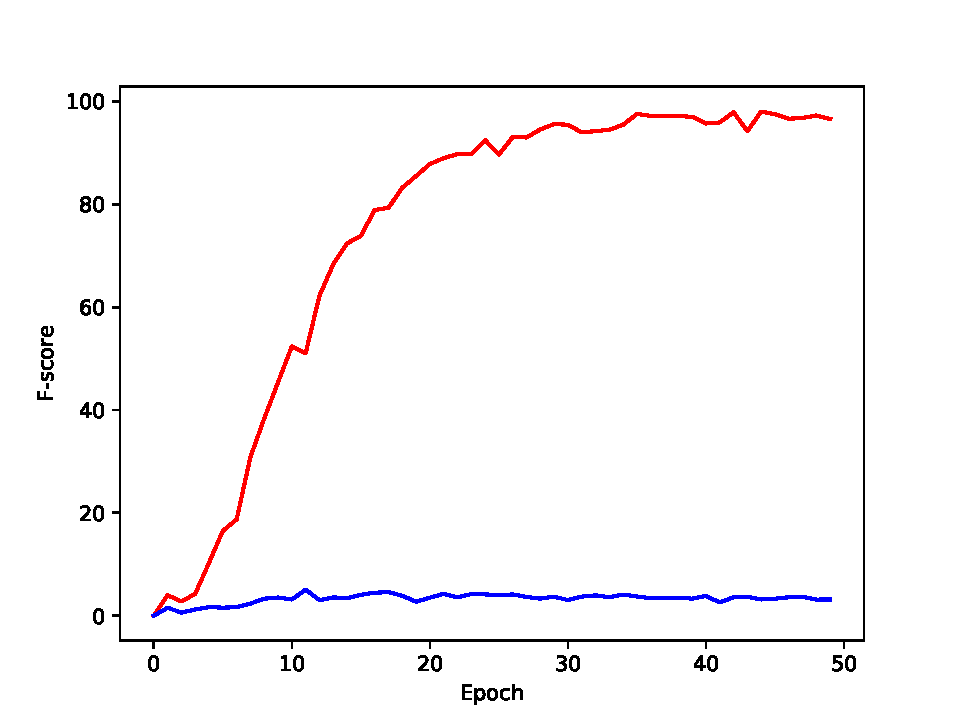
\includegraphics[width=0.7\columnwidth]{fig_lrn_0p001_atten_f.pdf}\caption{Greedy Search Decoding F-Score}\end{subfigure} \\

% \begin{subfigure}{0.4\textwidth}\centering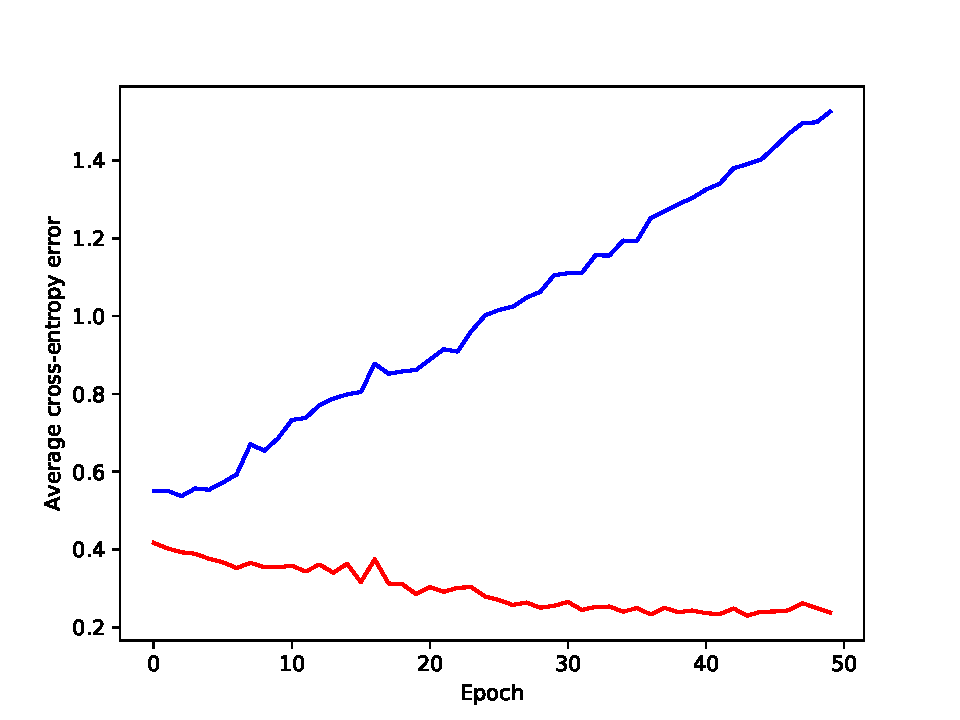
\includegraphics[width=0.7\columnwidth]{fig_lrn_0p001_beam_3_loss.pdf}\caption{Beam Search Decoding Loss}\label{fig:tabc}\end{subfigure} %\&
% \begin{subfigure}{0.4\textwidth}\centering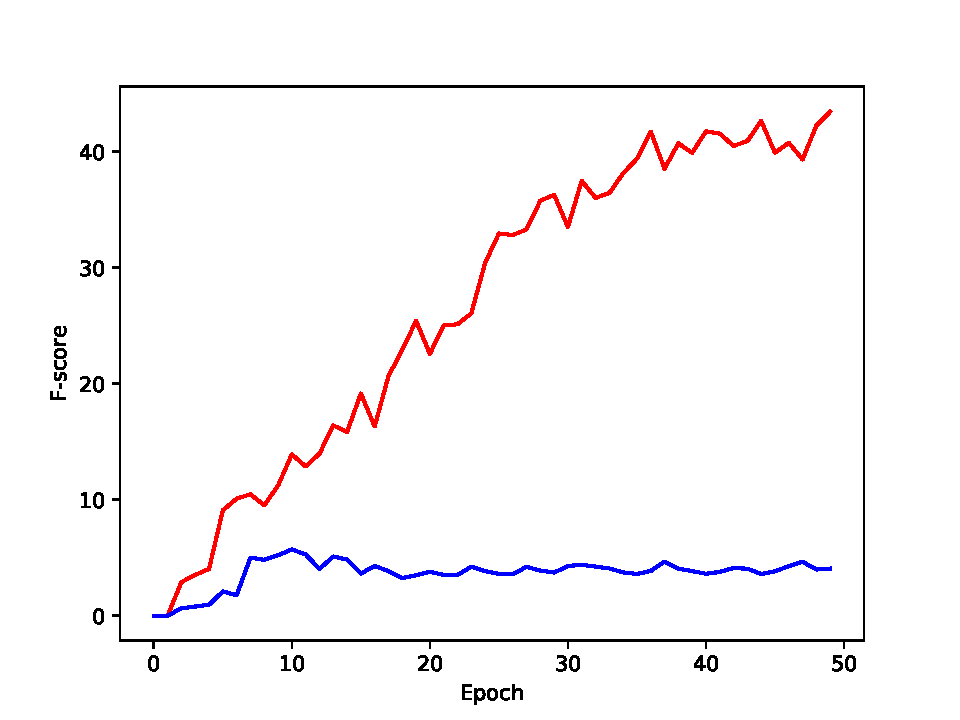
\includegraphics[width=0.7\columnwidth]{fig_lrn_0p001_beam_3_f.pdf}\caption{Beam Search Decoding F-Score}\label{fig:tabd}\end{subfigure} \\
% \captionof{figure}[]{The cross-entropy losses and F-scores of greedy search decoding \textbf{with attention}. Red curve is training set, and blue curve is validation set. Learning rate is 0.001. }
% \label{fig:attn_losses_fscore}
% \end{table*}
% % ========================================================================================================
% ========================================================================================================

% \begin{figure}[ht]
% \centering
% 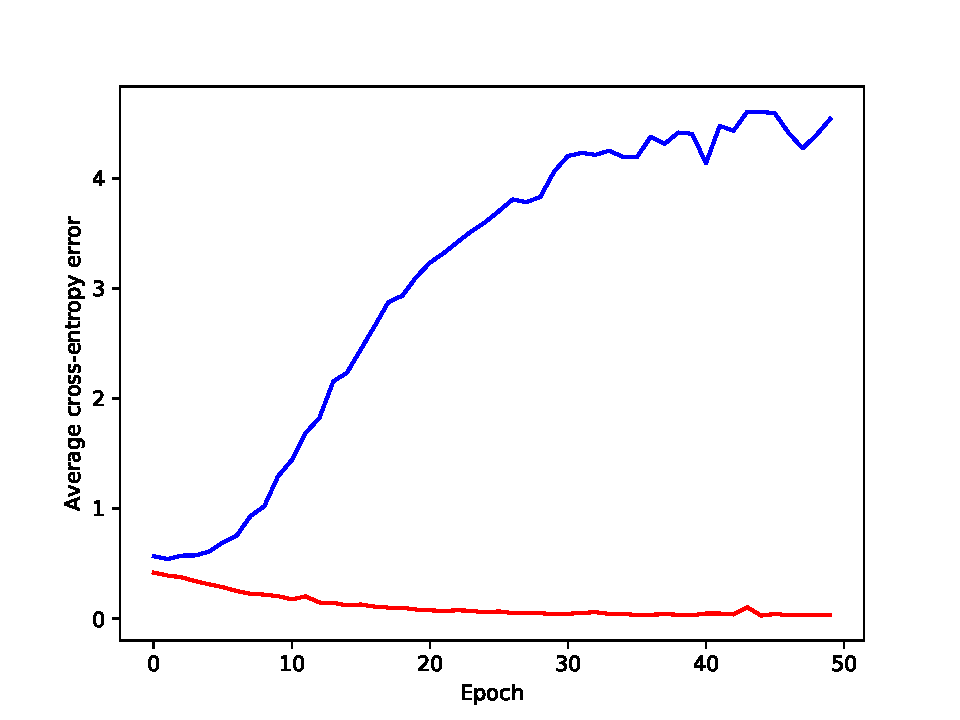
\includegraphics[width=0.8\linewidth]{fig_lrn_0p001_atten_loss.pdf}
% \caption{The cross-entropy loss with attention. Greedy decoding. Red curve is training set, and blue curve is validation set. Learning rate is 0.001.}
% \label{fig:fig_lrn_0p001_atten_loss}
% \end{figure}

% \begin{figure}[ht]
% \centering
% 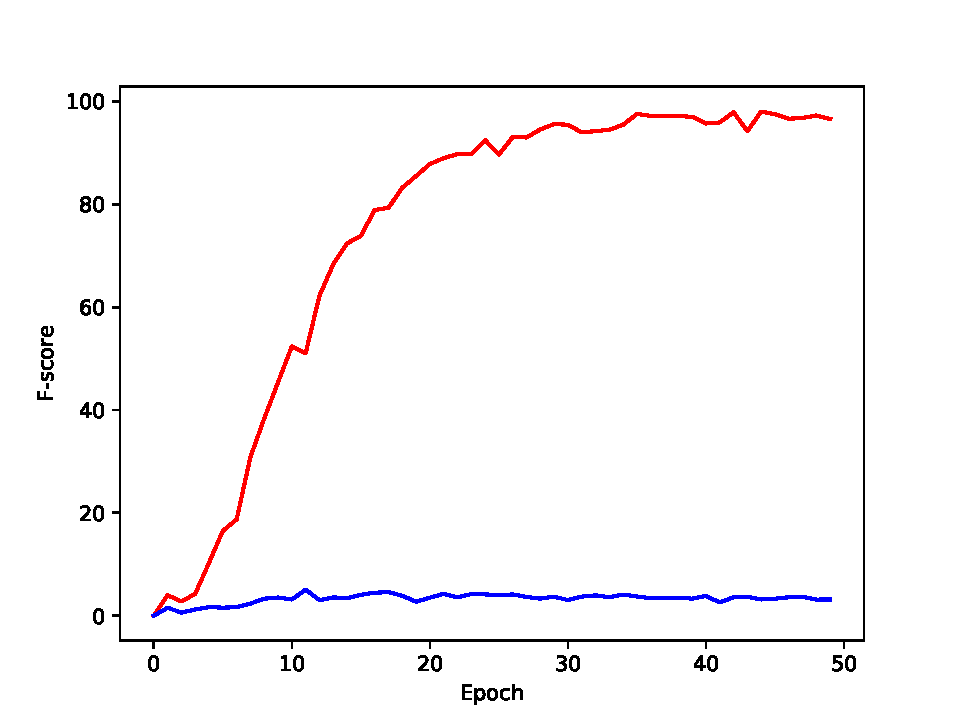
\includegraphics[width=0.8\linewidth]{fig_lrn_0p001_atten_f.pdf}
% \caption{The F-score with attention. Greedy decoding. Red curve is training set, and blue curve is validation set. Learning rate is 0.001.}
% \label{fig:fig_lrn_0p001_atten_f}
% \end{figure}




% \subsubsection{Extra penalization of non-``O'' class}

% 	As analyzed in assignment 1, the label distribution is skewed toward the label ``O''; that is, there are much more words with label O than there are with other labels. Since label O refers to ``not belonging to one of the NER class'', these words are not our primary learning targets. However, since they dominate the dataset, the model would naturally receive stronger learning signals from these instances. To encourage the model to learn more from the instances with labels other than O, we do the following extra penalization trick. For the instances whose true label is not O, we add extra points (we use 1.5) to the O's component of the score vector predicted by our model. In this way, the model is forced to generate prediction that much more strongly favors the non-O labels in order to overcome the penalization added to the O component.


% \subsubsection{Different Optimizers}

% Pytorch has API for most commonly used optimizers. The default optimizer we use for the previous experiments is Adam Optimizer. In this section, we tried three other optimizers - RMSprop, SGD, and Adagrad. The results of comparisions are shown in Table \ref{opti}. From the table, we can see different optimizers do not make much differences. Thus we stick to Adam Opitimizer for all experiments we conduct. 

    
% \begin{table}[ht]
% \centering
% \caption{After 30 epoches, the results of train data using different optimizers.}
% \label{opti}
% \begin{tabular}{llll}
% \hline
% Optimizer        & CE loss & Accuracy & F score \\ \hline
% Adam    & 0.1377  & 94.21\%  & 46.84   \\
% RMSprop & 0.1845  & 91.35\%  & 29.82   \\
% SGD     & 0.1488  & 93.37\%  & 41.26   \\
% Adagrad & 0.1363  & 93.89\%  & 47.38   \\ \hline
% \end{tabular}
% \end{table}



%\subsection{Parameter Tuning} \label{ssec:paratune}

%Before we start to experiment on the new search algorithms to improve the training and decoding of the seq2seq model, we first explore the effect of the choices of the hyperparameters on the performance of the neural networks. The hyperparameters we investigate are the batch size, the learning rate, the dimension of the word embeddings, and the number of the hidden units of the encoder. Once the parameter tuning is done, we plan to use pre-trained model for transfer learning and further fine tuning.


%\subsection{Comparison with the paper baseline}

% We compare our experimental result with the paper baseline from \cite{goyal2017continuous}. In particular, we compare with the Greedy Search and Hard Beam Search F-score of the NER task in Table 2 in \cite{goyal2017continuous}. Our experiment that is used for comparison uses beam size 3 and fixed attention. The result is given in Table \ref{tab:comp}.

% \begin{table}[ht]
% \centering
% \caption{Comparison of the F-score between our experiment and \cite{goyal2017continuous} at the NER task.}
% \label{tab:comp}
% \begin{tabular}{lrr}
% \toprule
%                   & F-score  & F-score    \\
%                   & (train)  & (val)    \\ \midrule
% Our greedy search          & 96.60            & 3.14               \\
% \cite{goyal2017continuous} greedy  & N/A              & 50.21              \\
% Our beam search          & 78.78            & 3.87               \\
% \cite{goyal2017continuous} beam  & N/A              & 46.22              \\ \bottomrule
% \end{tabular}
% \end{table}



% \subsection{Error analysis}

% From the results in Table \ref{tab:comp}, we get good F-scores for train data. 

% Currently we conducted 5 experiments on the NER tasks. The basic model has hyperparameter settings of $batch\_size=16$, $learning\_rate = 0.1$, $dim\_word\_embed =100$, and $hidden\_units=64$. For each experiments, we run 300 iterations due to the limited time. Figure \ref{fig:fig_exp1} shows the cross-entropy loss of the training data of the NER task over 300 iterations. 

% \begin{figure}[ht]
% \centering
% 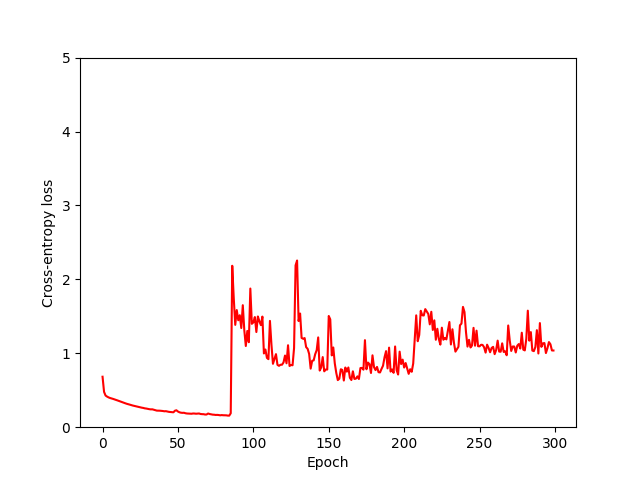
\includegraphics[width=0.8\linewidth]{fig_exp1.png}
% \caption{The training cross-entropy loss using the simple model for the NER task.}
% \label{fig:fig_exp1}
% \end{figure}

% % Please add the following required packages to your document preamble:
% % 
% \begin{table*}[ht]
% \centering
% \caption{Results of the Named Entity Recognition experiment. The first four columns are the parameters of each model, and the last two columns are the F-scores on the training data and the development data.}
% \label{f1table}
% \begin{tabular}{@{}cccc|cc@{}}
% \toprule
% batch size & learning rate & hidden units & dim\_word\_embed & F-score (train) & F-score (dev) \\ \midrule
% 16         & 0.1           & 64           & 100              & 1.64             & 1.52           \\
% 16         & 0.01          & 64           & 100              & 5.36             & 1.58           \\
% 32         & 0.01          & 64           & 100              & 13.13            & 1.24           \\
% 32         & 0.01          & 128          & 100              & 17.45            & 5.85           \\
% 32         & 0.01          & 128          & 200              & 3.44             & 2.63           \\ \bottomrule
% \end{tabular}
% \end{table*}

% \begin{table}[ht]
% \centering
% \caption{The precision, recall and F-score of the best model on train data for the NER task. Note that the tags in the table are not completely the same as the labels we use in the experiments. These labels are for evaluation purpose.}
% \label{precision}
% \begin{tabular}{@{}cccc@{}}
% \toprule
% Tag            & Precision        & Recall           & F-score       \\ \midrule
% LOC              & 37.53\%          & 8.22\%           & 13.49          \\
% MISC             & 18.96\%          & 4.18\%           & 6.85           \\
% ORG              & 58.32\%          & 23.10\%          & 33.10          \\
% PER              & 16.40\%          & 8.95\%           & 11.58          \\ \midrule
% \textbf{Overall} & \textbf{33.05\%} & \textbf{11.86\%} & \textbf{17.45} \\ \bottomrule
% \end{tabular}
% \end{table}



% \begin{table*}
% \renewcommand\thetable{1}
% \begin{center}
% \begin{tabular}{l|c|c|c|c}
% \hline
% Tag & Precision(\%) & Recall(\%) & F-score\\
% \hline\hline
% avg & 80.03 & 33.05 & 11.86 & 17.45 \\
% \hline
% LOC & 37.53 & 8.22 & 13.49 & 1524\\
% MISC & 18.96 & 4.18 & 6.85 & 733 \\
% \hline
% \end{tabular}
% \end{center}
% \caption{NER baseline result}
% \label{tbl:ner_baseline}
% \end{table*}

% We also report performance of different parameter settings on train data and development data sets for NER tasks in Table \ref{f1table}. Starting from the basic model, we try several values for each hyper-parameters and report the F1 scores using the official CONLL-2003 evaluation tool \cite{tjongkimsang2003conll}. Table \ref{precision} records the precision, recall and F1 score of the best model found in Table \ref{f1table}. 

% For the CCG SuperTagging task, we perform a preliminary experiment with $batch\_size=32$, $learning\_rate = 0.05$, $dim\_word\_embed =50$, $dim\_label\_embed =10$ and $hidden\_units=64$


%%%%%%%%%%%%%%%%%%%%%%%%%%%%%%%%%
%          DISCUSSION           
%%%%%%%%%%%%%%%%%%%%%%%%%%%%%%%%%
% results 
%\section{Improvement Directions for Future Work} \label{sec:discussion}% of baseline 
% discussion of results 

% \begin{figure}[ht]
% \centering
% %\fbox{\rule{0pt}{2in} \rule{0.9\linewidth}{0pt}}
%    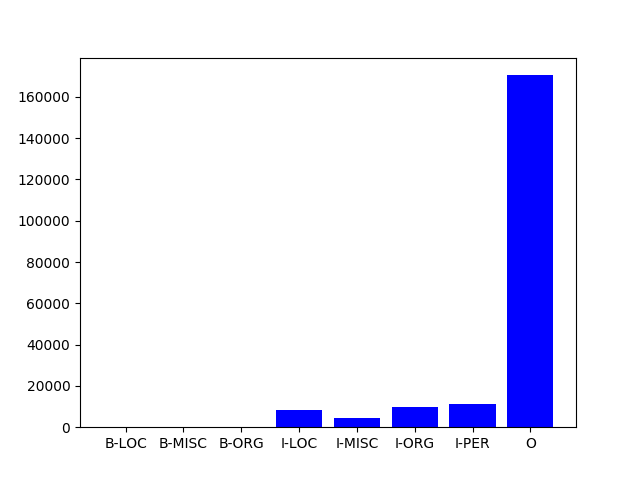
\includegraphics[width=0.8\linewidth]{NER_groundtruths.png}
%    \caption{Entity distribution of the CONLL-2003 NER dataset. Tag 'O' is overly dominant.}
% \label{fig_ner_gt}
% \end{figure}

% xAs seen in Figure~\ref{fig_ner_gt}, the dataset is largely skewed, particularly to the tag 'O', which makes the task hard. Empirically, we find the following trend from Tables \ref{f1table} and \ref{precision}:
% \begin{enumerate}
% 	\item The loss function value decreases faster when using some smaller batch size (we found the batch size of 16 works well). This can be understood by realizing that, with smaller batch size, we perform more updates within one epoch, therefore improving the loss decreasing rate per epoch. However, if the batch size is too small, the training speed will become much slower.
%     \item Larger dimension for the hidden state helps. This is expected because with large hidden dimension more context is remembered to be passed from the encoder to the decoder. Since we do not use attention in this assignment, we heavily rely on the hidden state to deliver all the information in the input sequence.
%     \item Using smaller learning rate for the SGD can be helpful. In Figure \ref{fig:fig_exp1} we observe that the loss function tends to be unstable at the later epochs of training. We found that by using smaller learning rate we can usually have more epochs that have stable training curve. However, if the learning rate is too small, the training process will also become too slow.
%     \item We find in our experiments that using smaller size of word embedding dimension (e.g.~around 100) seems to lead to better performance. At this stage we have not identified the reason for this phenomenon or whether this is really a general trend.
% \end{enumerate}




% We find that our F-score is much lower than the baseline number shown in \citet{goyal2018continuous}. In addition, from Figure \ref{fig:fig_exp1} we notice that the training loss curve becomes unstable at later epochs. To improve the F-score and the training process, we find many possible directions to pursue:

% \begin{enumerate}
% 	\item \emph{Use bi-directional LSTM for encoder.} We currently only use the single direction LSTM for encoder. To capture the context better, we can use bi-directional LSTM for encoder in the future.
%     \item \emph{Add attention mechanism.} In the task such as NER, even if there is only some fixed attention applied, the result is likely to be improved. This is because the named entity type of each word in the input sequence is mostly determined by the word itself (from human experience).
%     \item \emph{Add general beam search (not just greedy search).} Currently in test-time decoding we only implemented the greedy search, which is only a special case of the general beam search (with beam size of 1). With adjustable beam size can potentially improve the search results.
%     \item \emph{Experiment on different optimizers.} We use the vanilla SGD optimizer in this assignment. Without suitably adjusting the learning rate dynamically, it is likely that our training saturates at some point during the training process, and cannot improve the F-score or accuracy. We can try to dynamically adjust the learning rate or use different optimizers to see whether the training process would improve.
%     \item \emph{Be aware of the exploding gradient (or also the vanishing gradient) problem.} We noticed the instability of the training loss curve. We plan to check whether it is caused by the exploding gradient problem.
% \end{enumerate}
%\subsection{Error Analysis} \label{sec:improve}

% From the results in Table \ref{tab:comp}, Figures \ref{fig:no_attn_losses_fscore} and \ref{fig:attn_losses_fscore} we have a same pattern that the model yields a good performance for train data, but not the same for validation data. This behavior is apparently due to overfitting to training data, which is stemmed from not performing regularization such as dropout aggressively. 

% There are some strategies of dropout that we plan to apply to fix this. First, we can apply a normal dropout before and after embedding layer of inputs. This strategy can varies: we can apply a random mask based on position of a sentence or we can apply another mask on word basis (if a word is chosen to be deactivated, any of its occurrences will be gone). Second, we can apply dropout on the RNN cells on random time steps for encoder and decoder. And finally, we can apply the strategy such as in \cite{gal2016theoretically} where we can apply the same dropout patterns for input, recurrent and output for every single time step. We project that by using dropout properly, this overfitting situation will be mostly solved. 

% \subsection{Adaptive Beam Search} \label{sec:adaptive}

% We have addressed the basic concept of beam search and conducted some experiments on different beam size. For the final project, we will implement an adaptive beam search design. The original beam-search strategy generates the optimal prediction by approximately maximizing the conditional probability given by a Seq2seq model.  It builds the mapping from encoder-decoder and keeps a fixed number (beam) of candidates with the highest log-probability at each epoch. The search stops when the beam is full and the candidate with highest log-probability is picked from the candidate list. The problem of fixed-sized beam search is that all the candidates in the candidate list might not be the best possible scoring candidate, i.e. the best one is not added to the list before beam search stops. This issue can be avoided by increasing the beam size however it slows down the decoding speed. An adaptive beam search strategy can be much more flxible in terms of beam size at each epoch and do not increases the decoding time too much. Here is one possible design we come up with: Worse candidates pruning. This strategy discards those candidates in the candidate that are far worse than the best current candidate. In this case, we can keep beam size fixed, and continue pruning worst candidates to make space for next candidate. The pruning threshold can be various, e.g. relative threshold, abosulte threshold. We can tune it for the best performance. 








%%%%%%%%%%%%%%%%%%%%%%%%%%%%%%%%%
%          CONCLUSION           
%%%%%%%%%%%%%%%%%%%%%%%%%%%%%%%%%
\section{Conclusion} \label{sec:conclusion}
In this report we have demonstrated our improved seq2seq model with many new features, e.g. pre-trained word embeddings, bi-directional LSTM, beam search, attention and extra penalization. We have conducted experiments on NER tasks using our model, and the results of each experiments are shown and compared to the baseline as well. All the code is now made available in our github repository. 




% \begin{quote}
% \begin{verbatim}
% \usepackage{times}
% \usepackage{latexsym}
% \end{verbatim}
% \end{quote}
% in the preamble. If Times Roman is unavailable, use \textbf{Computer
%   Modern Roman} (\LaTeX2e{}'s default).  Note that the latter is about
%   10\% less dense than Adobe's Times Roman font.

% \begin{table}[t!]
% \begin{center}
% \begin{tabular}{|l|rl|}
% \hline \bf Type of Text & \bf Font Size & \bf Style \\ \hline
% paper title & 15 pt & bold \\
% author names & 12 pt & bold \\
% author affiliation & 12 pt & \\
% the word ``Abstract'' & 12 pt & bold \\
% section titles & 12 pt & bold \\
% subsection titles & 11 pt & bold \\
% document text & 11 pt  &\\
% captions & 11 pt & \\
% abstract text & 11 pt & \\
% bibliography & 10 pt & \\
% footnotes & 9 pt & \\
% \hline
% \end{tabular}
% \end{center}
% \caption{\label{font-table} Font guide. }
% \end{table}


% %Use 11 points for text and subsection headings, 12 points for section headings and 15 points for the title. 


% \begin{table}
% \centering
% \small
% \begin{tabular}{cc}
% \begin{tabular}{|l|l|}
% \hline
% \textbf{Command} & \textbf{Output}\\\hline
% \verb|{\"a}| & {\"a} \\
% \verb|{\^e}| & {\^e} \\
% \verb|{\`i}| & {\`i} \\ 
% \verb|{\.I}| & {\.I} \\ 
% \verb|{\o}| & {\o} \\
% \verb|{\'u}| & {\'u}  \\ 
% \verb|{\aa}| & {\aa}  \\\hline
% \end{tabular} & 
% \begin{tabular}{|l|l|}
% \hline
% \textbf{Command} & \textbf{ Output}\\\hline
% \verb|{\c c}| & {\c c} \\ 
% \verb|{\u g}| & {\u g} \\ 
% \verb|{\l}| & {\l} \\ 
% \verb|{\~n}| & {\~n} \\ 
% \verb|{\H o}| & {\H o} \\ 
% \verb|{\v r}| & {\v r} \\ 
% \verb|{\ss}| & {\ss} \\\hline
% \end{tabular}
% \end{tabular}
% \caption{Example commands for accented characters, to be used in, {\em e.g.}, \BibTeX\ names.}\label{tab:accents}
% \end{table}



% \begin{table*}
% \centering
% \begin{tabular}{lll}
%   output & natbib & previous ACL style files\\
%   \hline
%   \citep{Gusfield:97} & \verb|\citep| & \verb|\cite| \\
%   \citet{Gusfield:97} & \verb|\citet| & \verb|\newcite| \\
%   \citeyearpar{Gusfield:97} & \verb|\citeyearpar| & \verb|\shortcite| \\
% \end{tabular}
% \caption{Citation commands supported by the style file.
%   The citation style is based on the natbib package and
%   supports all natbib citation commands.
%   It also supports commands defined in previous ACL style files
%   for compatibility.
%   }
% \end{table*}



% include your own bib file like this:
%\bibliographystyle{acl}
%\bibliography{acl2018}
\bibliography{acl2018}
\bibliographystyle{acl_natbib}

% \appendix

% \section{Supplemental Material}
% \label{sec:supplemental}
% ACL 2018 also encourages the submission of supplementary material
% to report preprocessing decisions, model parameters, and other details
% necessary for the replication of the experiments reported in the 
% paper. Seemingly small preprocessing decisions can sometimes make
% a large difference in performance, so it is crucial to record such
% decisions to precisely characterize state-of-the-art methods.

% Nonetheless, supplementary material should be supplementary (rather
% than central) to the paper. \textbf{Submissions that misuse the supplementary 
% material may be rejected without review.}
% Essentially, supplementary material may include explanations or details
% of proofs or derivations that do not fit into the paper, lists of
% features or feature templates, sample inputs and outputs for a system,
% pseudo-code or source code, and data. (Source code and data should
% be separate uploads, rather than part of the paper).

% The paper should not rely on the supplementary material: while the paper
% may refer to and cite the supplementary material and the supplementary material will be available to the
% reviewers, they will not be asked to review the
% supplementary material.

% Appendices ({\em i.e.} supplementary material in the form of proofs, tables,
% or pseudo-code) should come after the references, as shown here. Use
% \verb|\appendix| before any appendix section to switch the section
% numbering over to letters.

% \section{Multiple Appendices}
% \dots can be gotten by using more than one section. We hope you won't
% need that.

\end{document}
